\def\Var{{\operatorname{Var}}\,}
\def\E{\mathbb{E}\,}

% custom tab cell
\newcommand{\bigcell}[2]{\begin{tabular}{@{}#1@{}}#2\end{tabular}}

% \input{../acronymsSorted.tex}
% \input{../myTikz.tex}

% color palette from https://coolors.co/e63946-3b1f2b-25ed91-457b9d-1d3557
\definecolor{desireRed}{RGB}{230,57,60}%
\definecolor{darkPurple}{RGB}{59,31,43}%
\definecolor{springGreen}{RGB}{37,223,145}%
\definecolor{queenBlue}{RGB}{69,123,157}%
\definecolor{spaceCadet}{RGB}{29,53,87}%

% Other palette
\definecolor{primaryColor}{HTML}{F06449}
\definecolor{secondaryColor}{HTML}{5BC3EB}
\definecolor{tertiaryColor}{HTML}{36382E}

\def\si{\tikz\fill[scale=0.4](0,.35) -- (.25,0) -- (1,.7) -- (.25,.15) -- cycle;}

% \usepackage[font=footnotesize]{caption}
% \usepackage[font=footnotesize]{subcaption}
% inherited from the template
% \def\BibTeX{{\mathrm B\kern-.05em{\sc i\kern-.025em b}\kern-.08em
%     T\kern-.1667em\lower.7ex\hbox{E}\kern-.125emX}}
    
%\setlength{\belowcaptionskip}{-0.5cm}
%\addtolength{\skip\footins}{-2mm}

%\section{Introduction}
%\label{sec:intro}

%With \gls{5g} networks ready for commercial deployment (it is expected that 5G will reach 1 billion users in 3 years), 

% The rest of the paper is organized as follows. 
% In Section~\ref{sec:ch_model_ext} we present a mathematical characterization of the channel for IRS/AF relays, based on the 3GPP channel model for 5G networks.
% Section~\ref{sec:simulator} describes our simulation methodology for IRS/AF relays. %with a focus on the modifications we made to the 3GPP channel model for 5G networks.
% In Section~\ref{sec:results} we show our main numerical results, while Section~\ref{sec:conclusion} concludes the work with suggestions for future research.


%The introduction of \glspl{irs} and \gls{af} relays will also require modifications of the 5G NR protocol stack, as well as  For example, the configuration of the IRS/AF beamforming vectors calls for a revised initial access and beam tracking procedure. Moreover, ad hoc signaling will also be required.

%TODO Say that no E2E simulators for smart EM are available. There exists a MATLAB simulator which is similar to ours, but it is not E2E (ony the channel is simulated by this work) \cite{9282349}

% The introduction of technologies such as \glspl{irs} and \gls{af} relays will necessarily require modifications in the 5G NR protocol stack. For instance, the configuration of the relays beamforming vectors calls for a revised initial access and beam tracking procedure. Moreover, ad-hoc signaling will also be required.

% Together with the ns-3 IAB module, this contribution allows researchers to compare in a realistic manner the performance of the most promising terrestrial relay technologies for 5G and 6G.

%TODO part of the following section can probably be moved to the introduction. 

%\section{End-to-End Simulation of \\ 5G Cellular Networks}
%\label{sec:model}
%TODO
%In recent years, simulation tools have been widely used to study the behavior of wireless networks.

%Furthermore, an ns-3 based \gls{ntn} simulator is being actively developed~\cite{puttonen2021system}, but at this moment in time no public release of the module is available either.

% \subsection{Channel models for \gls{5g} cellular networks simulators}
% An accurate channel model is a fundamental component of any system-level simulator~\cite{ferrand2016trends}. As such, the development of up-to-date channel models has been a hot research topic in recent years. In particular, most research efforts focused on the study of \glspl{mmwave} and beyond frequencies and \gls{mimo} systems~\cite{ferrand2016trends} channels.

% In order to adapt the previously sub-6 GHz only models to higher frequencies, various measurement campaigns have been conducted~\cite{zhao201328, maccartney2015indoor, deng201528}.
% % Maybe add something, like lower rank, different multipath fading and blockages.
% Moreover, the presence of large antenna arrays both at the transmitter and at the receiver called for the full 3D characterization of the channel, which in principle is different (but not independent) for each pair of antenna endpoints.
% These efforts have then jointly led to the development of a variety of novel channel models, each providing a different trade-off between physical accuracy and simulation scalability. For instance, \glspl{rt} can provide an accuracy which almost matches the one provided by traces obtained via measurement campaigns. However, they require a detailed description of the simulation scenario and they are particularly computationally intensive~\cite{lecci2020simplified}. 
% On the other hand, stochastic channel models such as the \gls{3gpp} TR~38.901~\cite{3gpp.38.901}, provide a more balanced trade-off between computational complexity, flexibility in the choice of the scenario and accuracy. Therefore, they usually represent the best option for system-level simulations.
% %measurement-based models offer the highest possible degree of fidelity, but they provide significant constraints on the simulation scenario, requiring the deployment to be fixed in advance in order to carry out measurement campaigns.
% \todo{Add more details on channel models in general ? }

% %Despite the wide range of available channel models, 
% To the best of our knowledge, none of these channel models have been extended to take into account the presence of passive and regenerative relays yet.
% Therefore, in the following section we propose and describe an extension of the \gls{3gpp} TR~39.901 channel model which introduces the support for passive and regenerative relays, i.e., entities such as \glspl{irs} and \gls{af} relay, and the modifications needed to the \gls{5g} NR protocol stack to support these devices.

 
\section{Modeling AF and IRS relays-aided wireless channels}
\label{sec:ch_model_ext}

Disruptive technologies, such as \glspl{irs} and \gls{af} relays, have been proposed as promising alternatives to overcome the coverage issues of \gls{mmwave} networks with energy efficiency in mind~\cite{flamini2022towards}. 
The former are meta-surfaces that can be programmed to favorably alter an \gls{em} field towards an intended destination. 
Most notably, \glspl{irs} are nodes which passively beamform the impinging signal, without amplification, thus being able to guarantee minimum capacity requirements in dead spots with lower power consumption compared to IAB~\cite{bjornson2019intelligent}. 
\Gls{af} relays, instead, are envisioned to capture an incident electromagnetic wave %through a phased array typically pointed towards
coming from a base station, to actively amplify the received signal, and to re-radiate it %by means of a second phased array that is pointed 
towards a target area to be served. They are candidates for achieving higher capacity with respect to IRS nodes, at the expense of higher cost and amplification noise~\cite{huang2019reconfigurable}.

Despite their research hype, whether these technologies will be able to fulfill 5G (and beyond) service requirements and, if so, how to properly dimension IRS/AF systems, are still crucial issues that remain unsolved. 
While field experiments with real hardware are infeasible due to scalability and flexibility concerns, as well as the high cost of testbed components, computer-based simulations represent a viable approach for testing and calibrating IRS/AF deployments. %solutions in 5G scenarios.
Prior works, e.g.,~\cite{wu2018intelligent,9282349}, have addressed this task, though focusing on link-level analyses, which typically adopt conservative assumptions on the system architecture, and should be taken as a lower bound for more representative end-to-end performance studies.
To fill this gap, in this section we provide a more comprehensive system-level performance evaluation of IRS/AF deployments using a new simulation
framework that operates end-to-end, thus incorporating the interplay with the \gls{5g} NR protocol stack and relative control tasks, as well as the impact of the upper (including transport and application) layers.
%Our framework is based on \mbox{ns-3}~\cite{ns3}, an open-source discrete-event simulator for wireless networks.

%A realistic characterization of the channel is the first step to obtain accurate simulation results. 
To this end, we first provide a mathematical model for the IRS and \gls{af} relay channels (Secs.~\ref{sec:irs_phy_model} and~\ref{sec:af_phy_model}, respectively), based on the standard 3GPP channel model for 5G networks (Section~\ref{sec:baseline_model}). % we describe the standard 3GPP channel model for 5G networks, and in Secs.~\ref{sec:irs_phy_model} and~\ref{sec:af_phy_model} we provide a mathematical model for the IRS and \gls{af} relay channels, respectively.

\emph{Notation.} We use boldface upper- and lower-case letters to refer to matrices and vectors, respectively, while lower-case letters denote scalars. We use $\bm{I}_{N}$ to denote the identity matrix of order $N$, $[ \bm{\Phi} ]_{j, k}$ to indicate the $(j, k)$-th
entry of matrix $\bm{\Phi}$, $\mathrm{diag} ( \phi_1,\dots, \phi_N) $ to indicate an $N$~$\times$~$N$ diagonal matrix with entries $\{\phi_j \, | \, j=1, \dots, N \}$. We use the superscripts T, H and~$*$ for transposition, Hermitian transposition, and conjugation, respectively.


%An accurate channel model is the underlying foundation of any system-level simulator. Accordingly, we begin the description of the proposed simulator by presenting an extension of the \gls{3gpp} TR~38.901 channel model which supports the presence of passive and regenerative relays between the communication endpoints. 

%First, we describe our baseline, i.e, the \gls{3gpp} TR~38.901 channel model and the ns-3 \texttt{mmwave} module, in Section~\ref{sec:baseline_model}. Then, we outline physically accurate models of both \glspl{irs} and \gls{af} relays in Sections~\ref{sec:irs_phy_model} and \ref{sec:af_phy_model}, respectively. 
%Then, we describe our baseline,  Section~\ref{sec:baseline_impl}. 
%Finally, we describe how to perform TR~38.901-based end-to-end simulations of passive and regenerative relays in Section~\ref{sec:ext_ch_model}.


\subsection{The TR~38.901 Channel Model for 5G NR}
 \label{sec:baseline_model}

Throughout this work, we consider the 3GPP TR~38.901 \gls{scm} standardized in~\cite{3gpp.38.901}, leaving the study of more accurate channel models (e.g., based on ray tracing measurements) as part of our future research.
 % in~\cite{zugno2020implementation}, and used in the \texttt{ns3-mmwave} module~\cite{mezzavilla2018end}. 
This choice is motivated by the fact that TR~38.901 supports a wide range of frequencies, from $0.5$ to $100$ GHz, and can be integrated with realistic beamforming models. Furthermore, it is suggested and adopted by the \gls{3gpp} itself for the performance evaluation of \gls{5g} networks via system-level simulations.

In particular, the TR~38.901 model outlines the procedures for generating a channel matrix $\bm{H}$ whose entries $\bm{H}_{p, q} (t, \tau)$ correspond to the impulse response of the channel between the $p$-th radiating element of the antenna array of the signal source (S), and the $q$-th radiating element of the antenna array of its destination (D), at time $t$ and with delay $\tau$. 
To model multipath fading, each of these terms is computed as the superposition of $N$ different clusters, each of which consists of $M$ rays that arrive (depart) to (from) the antenna arrays with specific angles and powers. Based on~\cite{3gpp.38.901}, and using the simplifications proposed in~\cite{zugno2020implementation}, the generic entry $\bm{H}_{p, q} (t, \tau)$ of the channel matrix can then be computed as:

\begin{equation}
\label{eq:ch_model_full_irs_sim}
\begin{aligned}
\bm{H}_{p, q}(t, \tau)=& \sum_{n=1}^{N} \sqrt{\frac{P_{n}}{M}} \sum_{m=1}^{M} \overline{\mathbf{F}}_{r x}\left(\theta_{n, m}^{A}, \phi_{n, m}^{A}\right) \\
& \times\left[\begin{array}{cr}
e^{j \Phi_{n, m}^{\theta, \theta}} & \sqrt{K_{n, m}^{-1}} e^{j \Phi_{n, m}^{\theta, \phi}} \\
\sqrt{K_{n, m}^{-1}} e^{j \Phi_{n, m}^{\phi, \theta}} & e^{j \Phi_{n, m}^{\phi, \phi}}
\end{array}\right] \overline{\mathbf{F}}_{tx}\left(\theta_{n, m}^{D}, \phi_{n, m}^{D}\right) \\
& \times e^{j \overline{\mathbf{k}}_{rx, n, m}^{T} \overline{\mathbf{d}}_{rx, p} e^{j \overline{\mathbf{k}}_{tx, n, m}^{T} \overline{\mathbf{d}}_{tx, q}}} e^{j 2 \pi v_{n} t} \delta\left(\tau-\tau_{n}\right).
\end{aligned}
\end{equation}
For a complete description of the specific terms appearing in Eq.~\eqref{eq:ch_model_full_irs_sim} we refer the interested reader to~\cite{zugno2020implementation}.

Then, a frequency-flat path gain term is added to each channel coefficient as a function of the carrier frequency $f_c$ and the distance $d$ between the endpoints, i.e., %Therefore, the same gain $\mathcal{P}_{L}$ is added to all the subcarriers within the \gls{psd} of the signal. 
%In line with~\cite{3gpp.38.901}, this path loss term is evaluated as:
\begin{equation}
\text{PL} (d, f_c) = A \log_{10} (d) + B + C \log_{10} (f_c) + X \, [\mathrm{dB}],
\label{eq:pl}
\end{equation}
where model parameters $A, B$ and $C$ depend on the propagation conditions and the type of environment, and $X$ is an optional term to represent shadowing~\cite{zugno2020implementation}. 

\begin{figure}[t]
  \centering
    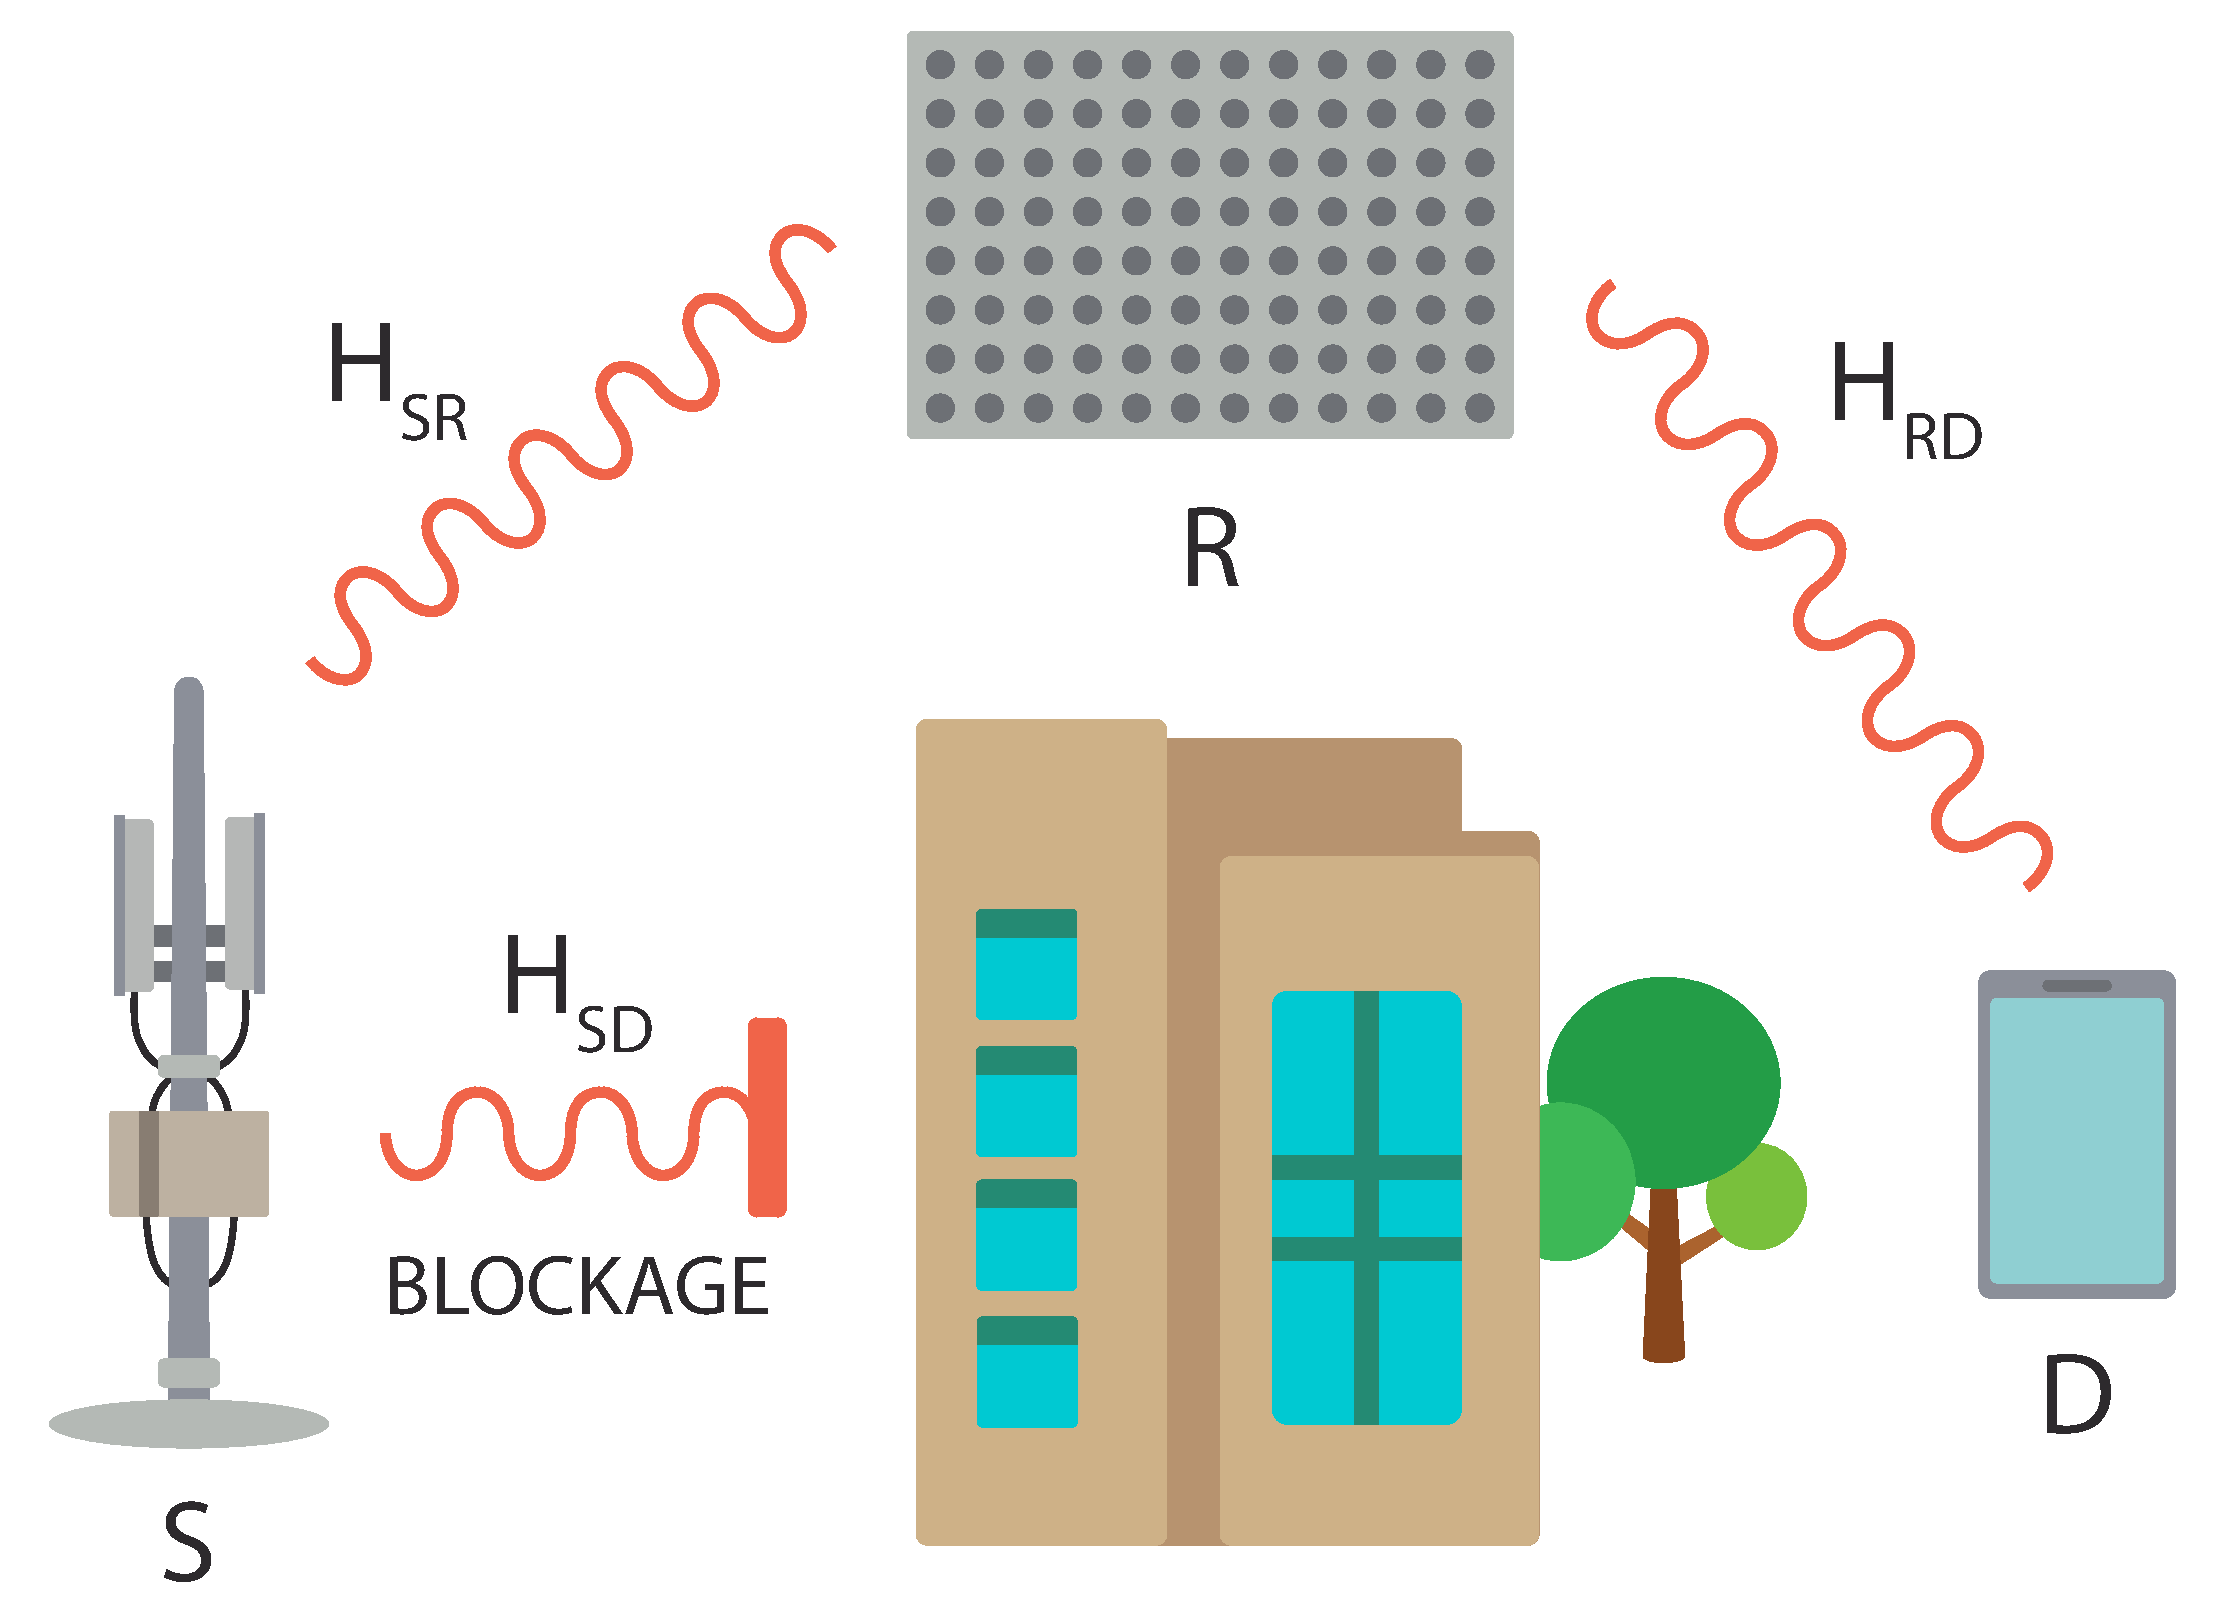
\includegraphics[width=0.75\textwidth]{Figures/IrsSimulation/Scenario_high_level.pdf}
  \caption{A typical urban scenario where a relay (R) can be used to bridge the signal from a source (S) to a destination (D), that would otherwise communicate in \acrshort{nlos}, i.e., the direct link between S and D is blocked due to obstacles such as buildings and/or vegetation.}
  \label{Fig:scenario_high_lvl}
\end{figure}

We consider the transmission of a single data stream $x_{\mathrm S}$, i.e., a sequence of signals, from a source S to a destination D via a relay R, as depicted in Figure~\ref{Fig:scenario_high_lvl}. 
Then, the channel matrix is combined with the beamforming vectors used at S and D, in order to obtain the \gls{sinr} experienced at D. 
In particular, let $x_{\mathrm S}$ be the signal transmitted from S to D, and $\bm{w}_{\mathrm S}$, $\bm{w}_{\mathrm D}$ and $\bm{w}_{\mathrm I}$ be the beamforming vectors used at S, D and the I-th interferer, respectively. Moreover, we define the following matrices:
$\bm{H}_{\mathrm SD}$ is the channel matrix between the source and the destination,
 $\bm{H}_{\mathrm ID}$ is the channel matrix between the \mbox{I-th} interferer and the destination,
 $\bm{H}_{\mathrm IR}$ is the channel matrix from the \mbox{I-th} interferer to the relay,
 $\bm{H}_{\mathrm SR}$ is the channel matrix between the source and the relay,
 and $\bm{H}_{\mathrm RD}$ is the channel matrix between the relay and the destination.
% $\bm{H}_{\mathrm SD}$ and $\bm{H}_{\mathrm ID}$ be the matrices of the S-D channel and the channel from the I-th interferer to D, respectively. 
In a relay-free environment, the signal received at the \gls{ue} is computed as:
\begin{equation}
    \label{eq:input_output_nodev}
    y_{\mathrm D} = \bm{w}_{\mathrm D}^{T} \bm{H}_{\mathrm SD} \bm{w}_{\mathrm S} x_{S} + \sum_{\mathrm{I}=1}^{N} \bm{w}_{\mathrm D}^{T} \bm{H}_{\mathrm ID}  \bm{w}_{\mathrm I} x_{\mathrm I} + \bm{w}_{\mathrm D}^{T} \bm{n}_{\mathrm D}.
\end{equation}
where $\bm{n}_D$ represents the circularly symmetric complex Gaussian noise vector with correlation matrix $\sigma_{\mathrm N}^2 \bm{I} $, and $\bm{w}_{\mathrm D}^{T} \bm{H}_{\mathrm ID} \bm{w}_{\mathrm I} x_{\mathrm I}$ is the signal received from the $\mathrm I$-th interferer.
Accordingly, the \gls{sinr} at D reads:
\begin{equation}
	\Lambda = \frac{ \lVert \bm{w}_{ \textrm D}^{T} \bm{H}_{\textrm {SD}}\bm{w}_{ \textrm S} \rVert^2 \sigma_{\mathrm S}^2 } { \sum_{\mathrm{I}=1}^{N} \lVert \bm{w}_{\mathrm D}^{T} \bm{H}_{\mathrm ID} \bm{w}_{\mathrm I} \rVert^2 \sigma_{\mathrm I}^2 + \sigma_{\mathrm N}^2 },
\end{equation}
where $\sigma_{\mathrm S}^2$ and $\sigma_{\mathrm I}^2$ are the powers of the intended and the $\mathrm{I}$-th interfering signals, respectively.
\subsection{A Signal Model for the IRS}
\label{sec:irs_phy_model} 
An \gls{irs} is a planar surface made of $N_{\mathrm R}$ low-cost passive reflecting elements that can be programmed to alter an \gls{em} field, for example to achieve three-dimensional beamforming towards an intended destination.
The working principle is similar to that of a conventional relay, the main difference being that while the latter amplifies the received signal before retransmitting it, an \gls{irs} reflects and beamforms the signal without introducing any amplification, thus saving power compared with other relaying solutions~\cite{bjornson2019intelligent}. %but promising lower gains as well. 


%However, in general the \gls{irs} is assumed to feature no signal processing capabilities.  

In particular, each element of the \gls{irs} acts as an 
%omnidirectional 
antenna that captures and reflects the incoming signals, introducing a phase shift on the baseband-equivalent signal. We denote with $\phi_n=e^{j\theta_n}, \, n = 1, \ldots, N_{\mathrm R}$, the reflection coefficient of the $n$-th \gls{irs} element, where $\theta_n \in [-\pi,\pi ] $ is the induced, controllable phase shift. 
Adopting a complex baseband notation, the signal $\bm{z} \in {\mathbb C}^{N_{\mathrm R} \times 1} $ reflected by an IRS (denoted as R), impinged with a signal $x_{\mathrm S}$ originating from a source S, reads
%When impinged with a signal $\bm{x}_{\mathrm S}$ originating from a source S, an \gls{irs} reflects the signal $\bm{z} \in {\mathbb C}^{N_{\mathrm R} \times 1} $, i.e.,
\begin{equation}
\bm{z}=\bm{\Phi}\bm{H}_{\mathrm SR} \bm{w}_{\mathrm S} x_{\mathrm S} ,
\end{equation}
%where $\bm{H}_{\mathrm SR}$ denotes the channel matrix between S and R, 
where $\bm{\Phi}$ is a diagonal matrix defined as $\bm{\Phi} \doteq \mathrm{diag} (\phi_1,\ldots,\phi_{N_{\mathrm R}})$, and typically referred to as {\em \gls{irs} configuration}. 
Therefore, the signal received at the intended destination D (under a far-field assumption with respect to the \gls{irs}) can be expressed as
\begin{equation}
	\label{eq:irs_iput_output}
    y_{\mathrm D} = \bm{w}_{\mathrm D}^{T} \bm{H}_{\mathrm RD} \bm{\Phi} \bm{H}_{\mathrm {SR}}  \bm{w}_{\mathrm S} x_S + \bm{w}_{\mathrm D}^{T} \bm{H}_{\mathrm SD} \bm{w}_{\mathrm S} x_S + \bm{w}_{\mathrm D}^{T} \bm{n}_{\mathrm D}.
\end{equation}
%where $\bm{H}_{\mathrm RD}$ denotes the matrix of the channel between the relay and the destination.
 
 \subsection{A Signal Model for the AF Relay}
 \label{sec:af_phy_model}
 
  \Gls{af} relays have been studied in the context of cooperative communications as a means to regenerate a relayed signal through amplification, with the goal of improving the system capacity. % And extending coverage?
  %The power amplifier entails that the gain of the AF relay is higher than that of a passive IRS when the number of IRS elements is equal to that of the AF relay antennas~\cite{huang2019reconfigurable}. On the downside, 
  Unlike \glspl{irs}, \gls{af} relays feature a non-negligible power consumption, and introduce noise amplification.

In this work we consider as \gls{af} relay a device equipped with $M_{\mathrm T}$ transmit and $M_{\mathrm R}$ receive antennas.
% two back-to-back panels of $M_{\mathrm R}$ antennas which first applies a receive beamforming vector $\bm{w}_{\mathrm R, RX}$ to obtain a single signal stream. Then, it amplifies and retransmits the latter using the transmit beamformer $\bm{w}_{\mathrm R, TX}$ and introducing an amplification $\mu_{\mathrm R}$. 
Therefore, the signal received at D is:
\begin{align}
\label{eq:af_iput_output}
    y_{\mathrm D} = \,\, &\bm{w}_{\mathrm D}^{T} \bm{H}_{\mathrm RD} \bm{\Phi} \bm{H}_{\mathrm {SR}} \bm{w}_{\mathrm S} x_{\mathrm S} + \bm{w}_{\mathrm D}^{T} \bm{H}_{\mathrm SD} \bm{w}_{\mathrm S} x_{\mathrm S}  \nonumber \\
   &+ \bm{w}_{\mathrm D}^{T} \bm{H}_{\mathrm RD} \bm{\Phi} \bm{n}_{\mathrm R} + \bm{w}_{\mathrm D}^{T} \bm{n}_{\mathrm D},
\end{align}
where in this case matrix $\bm{\Phi}$ also accounts for the amplification gain, and its structure depends on the specific relay design.
%\begin{equation}
%    \bm{\Phi} = \mu_{\mathrm R} \bm{w}_{\mathrm R, TX}  \bm{w}^T_{\mathrm R, RX}
%    \label{eq:phi_AF}
%\end{equation}
%is the rank-1 \gls{af} relay matrix obtained by multiplying the receive and transmit relay beamforming vectors $\bm{w}_{\mathrm R, RX}$ and $\bm{w}_{\mathrm R, TX}$, respectively. 
%Notice that, unlike for the \gls{irs}, matrix $\bm{\Phi}$ in~\eqref{eq:phi_AF} modeling the relay is not diagonal, since it is the result of the product of two beamforming vectors. 
Moreover, $\bm{n}_{\mathrm R}$ represents the circularly symmetric complex Gaussian noise vector with covariance matrix $\sigma_{\mathrm N_R}^2 \bm{I}_{M_{\mathrm R}} $.
Then, the power of the noise term relayed by the \gls{af} relay to receiver D and measured after the combiner at the \gls{ue}, is
\begin{equation} 
\label{eq:af_noise_power}
    \begin{split}
        \hat{\sigma}_{\mathrm N_R}^2 &= \left( \bm{w}_{\mathrm D}^{T} \bm{H}_{\mathrm RD} \bm{\Phi} \right) \left( \bm{w}_{\mathrm D}^{T} \bm{H}_{\mathrm RD} \bm{\Phi} \right)^{H} \sigma_{\mathrm N_R}^2 \\
         & = \bm{w}_{\mathrm D}^{T} \bm{H}_{\mathrm RD} \bm{\Phi} \bm{\Phi}^{H} \bm{H}_{\mathrm RD}^{H} {\bm w}^{*}_{\mathrm D} \sigma_{\mathrm N_R}^2.
    \end{split}
\end{equation}

%Furthermore, throughout this work we consider the \gls{af} relay to feature a \gls{pa} with a constraint on the maximum emitted power $P_{\mathrm max}$, due to saturation phenomena. 
%As such, $P_{\mathrm max}$ is a design parameter chosen a priori. 
%Moreover, we assume that the \gls{pa} has a maximum amplification factor $\mu_{\max}^2$.
%Under these assumptions, and using the above notation, the signal received at the %relay can be written as:
%\begin{equation}
%    y_{\mathrm R} = \bm{w}_{\mathrm R, RX}^{T} \bm{H}_{\mathrm {SR}} \bm{w}_{\mathrm S} x_{\mathrm S} + %\bm{w}_{\mathrm R, RX}^{T} \bm{n}_{\mathrm R}
%\end{equation}
%Then, assuming that the single-stream signal $x_{\mathrm S}$ has zero mean and variance $\sigma_{\mathrm S}^2$, the power of $y_{\mathrm R}$ can be expressed~as:
%\begin{equation}
%    P_{\mathrm R} = \left| \bm{w}_{\mathrm R, RX} ^{T} \bm{H}_{\mathrm {SR}} \bm{w}_{\mathrm S} \right|^2 \sigma_{\mathrm S}^2 + \sigma_{\mathrm N}^2.
%\end{equation}
%Thus, the amplification factor introduced by the relay is
%\begin{equation} \label{eq:af-amplif}
%    \begin{split}
%        \mu_{\mathrm R}^2 &= \min \left\{ \frac{P_{\mathrm max}}{ P_{\mathrm R}}, \, \mu_{\max}^2 \right\} \\
%        & = \min \left\{ \frac{P_{\mathrm max}}{\left| \bm{w}_{\mathrm R, RX}^{T} \bm{H}_{\mathrm {SR}} \bm{w}_{\mathrm S} \right|^2 \sigma_{\mathrm S}^2 + \sigma_{\mathrm N}^2}, \, \mu_{\max}^2 \right\}.
%    \end{split}
%\end{equation}

\subsection{A Full-Stack Simulator for IRS/AF Relays}
\label{sec:simulator}

Despite the availability of accurate sub-6 GHz and \gls{mmwave} channel models, analytical evaluations of the \gls{5g} NR protocol stack introduce several assumptions in the system architecture, and are generally not desirable~\cite{gkonis2020comprehensive}. 
%Moreover, \gls{5g} and beyond research is focusing on disruptive technologies, such as \glspl{irs}~\cite{8796365} and \glspl{ntn}~\cite{giordani2020non}, which are both extremely costly to test in the field, especially in their preliminary research phase.
Additionally, 5G/6G cellular networks are rapidly shifting towards open and controllable network configurations, which further introduce unprecedented data-driven programmability~\cite{bonati2020open}. 
In these regards, computer simulators are emerging as a valuable tool to let researchers better understand the performance of wireless networks, and dimension them accordingly~\cite{wilhelmi2021usage}.  

Several simulators for 5G cellular and vehicular networks are available in the literature~\cite{mezzavilla2018end,choi20195g, nardini2020simu5g, patriciello2019e2e, pratschner2018versatile, muller2018flexible, jao2018wise,drago2020millicar}. However, they provide a detailed characterization of either the lower (i.e., at the link level) or the upper (i.e., at the system level) layers of the \gls{5g} NR protocol stack. 
%Accordingly, they are typically referred to as link-level or system-level simulators, respectively. 
Notably, the latter sacrifice \gls{phy} layer accuracy to reduce the computational complexity, but incorporate accurate models of the remainder of the protocol stack, thus enabling scalable end-to-end simulations.
Despite the many software-based evaluation platforms available, to the best of our knowledge there are no end-to-end simulators for IRSs and AF relays. In~\cite{polese2018end}, the authors presented an open-source module for \gls{iab}, even though it was not extended to support passive relays like IRSs. 
Moreover, the authors in~\cite{heimann2021modeling} presented an ns-3 \gls{irs} module, but their work focused on vehicular networks, and did not consider the case of AF~relays. 
In this work we fill this gap by proposing an ns-3-based simulator for IRSs and AF relays.
Arguably, the main effect of the presence of these entities is the alteration of the wireless channel between the communication endpoints. 
%This implies that the \gls{sinr} experienced over such channel will also be different compared to the case where no relays are deployed. 
Accordingly, our simulator extends the \texttt{ns-3 mmwave} module~\cite{mezzavilla2018end} (among the most popular 5G-oriented NR-compliant frameworks to simulate 5G networks) by implementing a new signal model for IRS and AF relays, following the characterization in Secs.~\ref{sec:irs_phy_model} and \ref{sec:af_phy_model}, respectively, which is then used to compute the \gls{sinr} experienced by signals transmitted over a relayed wireless link. 

%the bulk of our simulator consists in the implementation of a channel model for IRS and AF relays, based on the characterization in Secs.~\ref{sec:irs_phy_model} and \ref{sec:af_phy_model}, which is then used to compute the \gls{sinr} experienced by signals transmitted over a relayed wireless link. 
\subsubsection{Implementation of the IRS/AF Signal Model} 
\label{sec:ext_ch_model}
 
In line with~\cite{zugno2020implementation}, we assume that the transmission of the signal $x_{\mathrm S}$ occurs over a frequency-selective wireless channel as \gls{5g} NR supports network operations with a bandwidth up to 400 MHz, when using FR2~\cite{38101_1}. 
Therefore, the evaluation of the \gls{sinr} requires, among other things, the computation of the \gls{psd} of the useful component of the signal at D, i.e., $\mathcal{P}_{r x}$, starting from that of the input signal $\mathcal{P}_{t x}$. Additionally, we consider that both the transmitter and the receiver feature \gls{m-mimo} arrays equipped with multiple antenna elements, and use the beamforming vectors $\bm{w}_{\textrm S}$ and $\bm{w}_{\textrm D}$, respectively.
Under these assumptions, the input-output relationship in~\eqref{eq:input_output_nodev} becomes~\cite{bjornson2019intelligent, wu2019intelligent}:
\begin{equation}
\label{eq:mimo_input_output_relay}
\begin{aligned}
	y_{D} = \,\, & \bm{w}_{\mathrm D}^{\mathrm T} \bm{H}_{\mathrm RD} \bm{\Phi} \bm{H}_{\mathrm {SR}} \bm{w}_{\mathrm S} x_{S} + \bm{w}_{\mathrm D}^{T} \bm{H}_{\mathrm SD} \bm{w}_{\mathrm S} x_{S} + \tilde{n} + \\
	& \sum_{\mathrm{I}=1}^{N} \bm{w}_{\mathrm D}^{T} \bm{H}_{\mathrm {RD}} \bm{\Phi} \bm{H}_{\mathrm {IR}}  \bm{w}_{\mathrm I} x_{\mathrm I} + \sum_{\mathrm{I}=1}^{N} \bm{w}_{\mathrm D}^{T} \bm{H}_{\mathrm ID}  \bm{w}_{\mathrm I} x_{\mathrm I},
\end{aligned}
\end{equation}
where in turn $\tilde{n}$ is defined as:
\[ 
\tilde{n} = 
\begin{cases}
    \bm{w}_{\mathrm D}^{T} \bm{n}_{\mathrm D}		& \text{if IRS}, \\
    \bm{w}_{\mathrm D}^{T} \bm{n}_{\mathrm D} + \bm{w}_{\mathrm D}^{T} \bm{H}_{\mathrm RD} \bm{\Phi} \bm{n}_{\mathrm R}      & \text{if AF},
\end{cases}
\]
where matrix $\bm{\Phi}$ is the relay matrix, i.e., a matrix which fully encodes the effect of the relay, i.e., either IRS or AF, as described in Secs.~\ref{sec:irs_phy_model} and~\ref{sec:af_phy_model} for the single user case, respectively, over the wireless channel. 
%The terms $\bm{H}_{\mathrm {SR}}$, $\bm{H}_{\mathrm {IR}}$, $\bm{H}_{\mathrm {RD}}$ represent the channel matrices between the source and the relay, the $\mathrm{I}$-th interferer and the relay, and the relay and the destination, respectively. Moreover, $\bm{H}_{\mathrm {SD}}$, $\bm{H}_{\mathrm {ID}}$ are the channel matrices of the direct link from the source and the $\mathrm{I}$- th interferer to the destination, as illustrated in Figure~\ref{Fig:scenario_high_lvl}.
Notably, S and D are either in \gls{nlos} (in this case they communicate via the relay, and we consider the direct link towards D to be unavailable), or in \gls{los} (in this case they do not use the relay). % thus we consider the secondary path reflected by such entity to be negligible.
%These assumptions are motivated by the fact that we envision as the main use case for these kinds of relays scenarios in which the direct path between S and D is almost completely blocked by obstacles, such as building and/or vegetation.
Accordingly, assuming that the source of interest is in NLOS with respect to its intended destination,~\eqref{eq:mimo_input_output_relay} becomes:

\begin{equation}
\label{eq:mimo_input_output_relay_reduced}
\begin{aligned}
    y_{D} = \,\, & \bm{w}_{\mathrm{D}}^{\mathrm{T}} \bm{H}_{\mathrm{RD}} \bm{\Phi} \bm{H}_{\mathrm{SR}} \bm{w}_{\mathrm{S}} x_{S} + \sum_{\hat{I} \in  I_{\mathrm{LOS}}} \bm{w}_{\mathrm{D}}^{T} \bm{H}_{\mathrm{\hat{I}} D} \bm{w}_{\mathrm{\hat{I}}} x_{\mathrm{\hat{I}}} \\
  & + \sum_{ \bar{I} \in I_{\mathrm{NLOS}}} \bm{w}_{\mathrm{D}}^{T} \bm{H}_{\mathrm{RD}} \bm{\Phi} \bm{H}_{\mathrm{\bar{I} R}}  \bm{w}_{\mathrm{\bar{I}}} x_{\mathrm{\bar{I}}} + \tilde{n},
\end{aligned}
\end{equation}
where $I_{\mathrm{LOS}}$ and $I_{\mathrm{NLOS}}$ are the two disjoint sets of interferers which experience either an \gls{los} or an \gls{nlos} channel towards D, respectively.
Then, the \gls{psd} of the useful component of the signal at the receiver can be written as:
\begin{equation}
\label{eq:psd_relay}
\mathcal{P}_{r x}(t, f) = \mathcal{P}_{t x}(t, f) \lVert \bm{w}_{\textrm D}^{\textrm T} \bm{H}_{\textrm {RD}} \bm{\Phi} \bm{H}_{\textrm {SR}} \bm{w}_{\textrm S} \rVert^2.
\end{equation}

Based on the above definitions, our simulator computes the \gls{psd} by checking whether the communication from S to D involves a relay. 
If so, the \gls{psd} is computed according to the following steps.

\begin{enumerate}
    \item \emph{Channel matrices generation.} 
%First of all, we identify the relay's antennas communicating towards S and D. 
%For the sake of using a general model tailored to both forms of relays (i.e., IRS and AF), we assume that R features two antenna arrays, possibly pointing to different directions. %Depending on the type of relay, these arrays might then coincide in practice. 
After having identified S and D as the two endpoints of the communication, the channel matrices $\bm{H}_{\textrm {SR}}$ and $\bm{H}_{\textrm {RD}}$ are computed based on~\eqref{eq:ch_model_full_irs_sim}~\cite{3gpp.38.901}. 

\item \emph{Configuration of the relay and beamforming vectors.}
We assume that the choice of the beamforming vectors for both S and D ($\bm{w}_{\textrm D}$ and $\bm{w}_{\textrm S}$), as well as the relay configuration ($\bm{\Phi}$), consist in the choice of a \emph{codeword} from a pre-defined \emph{codebook}. The latter is computed offline by first defining a set of beam directions $\{ \omega_{n, m} \}$ which scan a given angular sector via steps of \gls{hpbw}. In particular, let $\bm{a}_{n,m}$ be the steering vector corresponding to direction $\omega_{n, m}$. This is computed~as:
\medmuskip=1mu
\thinmuskip=1mu
\thickmuskip=1mu
\begin{equation}
\begin{aligned}
    \bm{a}_{n, m} & =  \left[ 1,\ldots, e^{j\frac{2\pi}{\lambda}d\left(i_{\mathrm H}\sin\alpha_n\sin\beta_m+i_{\mathrm V}\cos\beta_m\right)}, \ldots, \right. \\ 
    & \left. e^{j\frac{2\pi}{\lambda}d\left((N_{\mathrm H}-1)\sin\alpha_n\sin\beta_m+(N_{\mathrm V}-1)\cos\beta_m\right)}\right]^T,
\end{aligned}
\end{equation}
\medmuskip=6mu
\thinmuskip=6mu
\thickmuskip=6mu
where $0 \leq i_{\mathrm H} \leq N_{\mathrm H}$ ($0 \leq i_{\mathrm V} \leq N_{\mathrm V}$) is the horizontal (vertical) index of an antenna element, $N_{\mathrm H}$ and $N_{\mathrm V}$ are the number of antenna elements in the horizontal and vertical direction, respectively, and $\alpha_n$ and $\beta_m$ represent the azimuth and the elevation angles of $\omega_{n, m}$, respectively. Then, we define the codeboook for the \glspl{ue}, \glspl{gnb} and \gls{af} relays as the set $\{ \left( \sqrt{N_{\mathrm H} N_{\mathrm V}} \right)^{-1} \bm{a}_{n, m} \}$, while the \gls{irs} codebook is defined as $\{ \bm{a}_{n, m} \}$. 
%Notably, for the \gls{irs} codebook the normalization term $ \left( \sqrt{N_{\mathrm H} N_{\mathrm V}} \right)^{-1}$ is not present, since the power of any impinging signal must be completely re-radiated by each \gls{irs} element.

Moreover, we assume that the devices do not have full channel knowledge, i.e., they do not know the realizations of $\bm{H}_{\textrm {SR}}$ and $\bm{H}_{\textrm {RD}}$. 
Then, in line with the \gls{5g} NR beam management procedure~\cite{giordani2018tutorial}, the choice of the codeword in the codebook is performed via exhaustive search, i.e., by repeatedly sending pilot signals, and measuring the \gls{sinr} experienced with various configurations of the codebook. Eventually, we choose the combination of $\bm{w}_{\textrm D}$, $\bm{w}_{\textrm S}$, and $\bm{\Phi}$ yielding the highest \gls{sinr}.

Notably, this procedure is not repeated at each transmission opportunity. Instead, $\bm{w}_{\textrm D}$, $\bm{w}_{\textrm S}$, and $\bm{\Phi}$ are stored and re-used for the whole channel coherence time, to mimic the actual 5G NR beam management procedure, and also reduce the complexity of the simulations. 
Furthermore, the evaluation of the \gls{sinr} is performed by neglecting the small-scale fading terms, to further reduce the overhead. The small-scale fading will be eventually incorporated in Step 4 of the model.

\item \emph{Long-term computation.} 
%The computation of the \gls{psd} at the receiver is decomposed into two sub-parts, . As such, 
%by explicitly outlining the vector and matrices products of Eq.~\ref{eq:psd_relay} 
Along the lines of~\cite{zugno2020implementation}, the \gls{psd} of the transmitted signal $x_S$ at D can be expressed as:
\begin{equation}
\begin{aligned}
&\mathcal{P}_{r x}(t, f) = \\
& = \mathcal{P}_{t x}(t, f) \lVert \bm{w}_{\textrm D}^{\textrm T} \bm{H}_{\textrm {RD}} \bm{\Phi} \bm{H}_{\textrm {SR}} \bm{w}_{\textrm S} \rVert^2 \\
&=\mathcal{P}_{t x}(t, f) \lVert \bm{w}_{\textrm D}^{\textrm T} \bm{H}_{\textrm {SRD}} \bm{w}_{\textrm S} \rVert^2 \\
& = \mathcal{P}_{t x}(t, f) \left\lVert \sum_{d=1}^{N_D} \sum_{s=1}^{N_S}  w^{\textrm D}_{d} h^{\mathrm SRD}_{d, s} (t, f)  w^{\textrm S}_{s} \right\rVert^2.
\end{aligned}
\label{eq:p-rx-sdr}
\end{equation}

In Eq.~\eqref{eq:p-rx-sdr}, $\bm{H}_{\mathrm SRD}$ is the equivalent channel matrix between S and D, whose generic entry $h^{\mathrm SRD}_{d, s} (t, f)$ is:
\begin{equation}
\begin{aligned}
\label{eq:psd_relay_sums}
h^{\mathrm SRD}_{d, s} (t, f) &= \left[ \bm{H}_{\textrm {RD}} (t, f) \bm{\Phi} \bm{H}_{\textrm {SR}} (t, f) \right]_{d, s} \\
& = \sum_{n=1}^{N_{\mathrm RD}} \sum_{m=1}^{N_{\mathrm SR}} \sum_{k=1}^{N_{R}} \sum_{l=1}^{N_{\mathrm R}} h^{\mathrm RD}_{d, k, n} \, \phi_{k, l} \, h^{\mathrm SR}_{l, s, m} \\
& \quad \times e^{j 2 \pi v_{n} t} e^{j 2 \pi \tau_{n} f} \\
& \quad \times e^{j 2 \pi v_{m} t} e^{j 2 \pi \tau_{m} f},
\end{aligned}
\end{equation}
where $N_{\mathrm RD}$ and $N_{\mathrm SR}$ are the number of multipath clusters in $\bm{H}_{\textrm {RD}}$ and $\bm{H}_{\textrm {SR}}$, respectively. Moreover, $w^{\textrm S}_{s}$ and $w^{\textrm D}_{d}$ denote entries $s$ and $d$ of vectors $\bm{w}_{\mathrm S}$ and $\bm{w}_{\mathrm D}$, respectively.
Then, Step 3 consists in the evaluation of the long-term fading:
\begin{equation}
L_{n, m} \doteq \sum_{d=1}^{N_{\mathrm D}} \sum_{s=1}^{N_{\mathrm S}} \sum_{k=1}^{N_{\mathrm R}} \sum_{l=1}^{N_{\mathrm R}} w^{\mathrm D}_{d} \, h^{\mathrm RD}_{d, k, n} \, \phi_{k, l} \, h^{\mathrm SR}_{l, s, m} \, w^{\mathrm S}_{s}. 
\end{equation}
%which involves the terms in the summations of Eq.~\eqref{eq:psd_relay_sums} which vary relatively slowly over time only.

\item \emph{Small-scale fading and path loss.}
The small-scale fading terms are combined with the terms $L_{n, m}$ to compute the overall fading component of the \gls{psd} of interest:
\begin{equation}
	\mathcal{\tilde{P}}_{rx}(t, f) = \mathcal{P}_{t x}(t, f) \left\lVert \sum_{n=1}^{N_{\mathrm RD}} \sum_{m=1}^{N_{\mathrm SR}} L_{n, m} E_{n, m}  \right\rVert^2,
\end{equation}
% A bit tedious to read, but could not fit in a single line otherwise..
where
\begin{equation}
E_{n, m} \doteq e^{j 2 \pi v_{n} t} e^{j 2 \pi \tau_{n} f} e^{j 2 \pi v_{m} t} e^{j 2 \pi \tau_{m} f}.
\end{equation}
Additionally, the path loss is computed as in~\eqref{eq:pl}. Since the useful signal received at D experiences two channels (from S to R, and from R to D) as a cascade, as described in~\eqref{eq:mimo_input_output_relay}, two path loss terms are added (in dB), to obtain the final \gls{psd} of $x_S$ at D as:
\begin{equation}
\begin{split}
\mathcal{P}_{r x}(t, f)& [\mathrm{dB}]  = \text{PL} (d_{\mathrm{SR}}, f_c) [\mathrm{dB}] \\
& + \text{PL} (d_{\mathrm{RD}}, f_c) [\mathrm{dB}] + \mathcal{\tilde{P}}_{rx}(t, f) [\mathrm{dB}].
\end{split}
\end{equation}
\item \emph{Interference and \gls{sinr}.}
As the last step, we evaluate the \glspl{psd} $\{ \mathcal{P}_{i}(t, f) \}_{i = 1, \dots, N_I}$ of the $N_I$ interfering signals at D. %The same assumptions are introduced, i.e., for \gls{los} (\gls{nlos}) devices the relayed (direct) link is neglected. 
To do so, we follow Steps 1--4 as for the useful component of the signal. However, the beamforming configurations are not optimized as described in Step 2. That is to say, each interferer uses the beamforming vector yielding the highest \gls{sinr} \emph{towards its intended destination}, while R and D employ the same configurations used in the previous steps.
Finally, the \gls{sinr} is evaluated as:
\[ \Lambda (t, f) = \frac{ \mathcal{P}_{r x}(t, f)} {\sum_{i=1}^{N_I} \mathcal{P}_{i}(t, f) + \mathcal{P}_{n}(t, f) },  \]
where $\mathcal{P}_{n}(t, f)$ is the \gls{psd} of the thermal noise at D.
\end{enumerate}

\subsubsection{Integration of the IRS/AF Signal Model in the Simulator}
In Section~\ref{sec:ext_ch_model} we described how our simulator computes the channel (in terms of \gls{psd}) in case of IRS/AF relays, which is then used to calculate the end-to-end SINR at the destination D. 
Notice that the \gls{sinr} can refer to either the \gls{sinr} relative to the whole bandwidth, for narrowband signals over frequency-flat channels, or the \gls{sinr} experienced over a single subcarrier, for wideband signals transmitted over frequency-selective channels. 
In the second case, the \glspl{sinr} corresponding to the various frequency chunks are then mapped into a single \gls{sinr} value, according to additional maps obtained from link-level simulations~\cite{lagen2020new}.
Based on that, our simulator defines a \gls{l2sm}, i.e., a table which associates a given \gls{sinr} to a \gls{mac}-layer \gls{tb} error rate~\cite{mezzavilla2012lightweight}, in turn used to decide whether the \gls{tb} has been correctly received or not.
%At each transmission opportunity, the \gls{sinr} is computed, by simulating the wireless channel and possibly combining it with transmit and receive beamforming vectors.
%Finally, the \gls{l2sm} is used to map such \gls{sinr} to the error probability of the corresponding \gls{mac} \gls{tb} and, .

The upper layers of the 5G NR protocol stack are modeled based on the \texttt{ns3-mmwave} module~\cite{mezzavilla2018end}, which implements a custom \gls{phy} layer supporting the NR frame structures and numerologies, and a \gls{mac} layer with ad hoc beamforming and scheduling policies. 
The \gls{rlc} and \gls{pdcp} layers implement network functions such as packet segmentation, retransmissions and/or reassembly. 
\begin{figure}[t!]
  \centering
    \begin{subfigure}[t]{\columnwidth}
    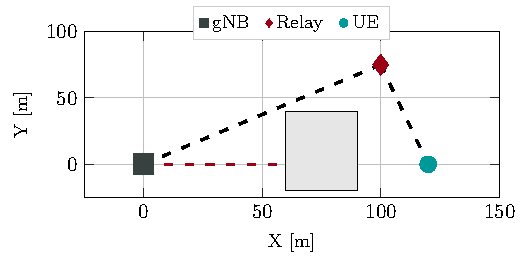
\includegraphics[width=0.75\columnwidth]{Figures/IrsSimulation/Scenario1.pdf}
    \caption{Scenario 1, with $N_{\mathrm U} = 1$.}
    \label{Fig:s1}
    \end{subfigure}
     \begin{subfigure}[t]{\columnwidth}
    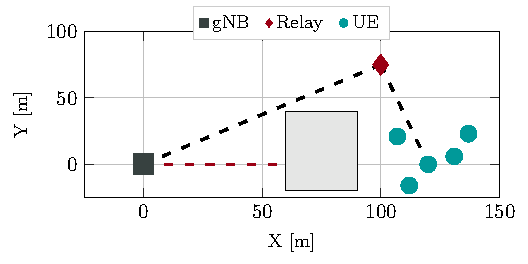
\includegraphics[width=0.75\columnwidth]{Figures/IrsSimulation/Scenario2.pdf}
    \caption{Scenario 2, with $N_{\mathrm U} = 5$.}
    \label{Fig:s2}
    \end{subfigure}
     \caption{Simulation scenarios, where we deploy one \gls{gnb}, $N_{\mathrm U}$ \glspl{ue} and, possibly, a relay. A building (the gray rectangle) blocks the direct link (dashed red line) from the \gls{gnb} to the \glspl{ue}. In turn, the relay guarantees a \gls{los} link (dashed black line) to all the devices.}
    \label{Fig:scenarios}
\end{figure}

\subsection{Performance Evaluation}
\label{sec:results}

In this section we describe our simulation setup and parameters (Section~\ref{sub:simulation_setup}), and evaluate the performance of \glspl{irs} and \gls{af} relays, considering full-stack network metrics as a function of different antenna array configurations (Section~\ref{sub:numerical_results}).

\subsubsection{Simulation Setup} % (fold)
\label{sub:simulation_setup}

In our simulations we consider two simple yet realistic urban canyon scenarios, where we deploy a single \gls{gnb}, $N_{\mathrm U}$ \glspl{ue}, with $N_{\mathrm U}=1$ (5) in Scenario 1 (2), as illustrated in Figure~\ref{Fig:scenarios}, and a single relay, which can be either an \gls{irs} or an \gls{af} relay.
The wireless channel is modeled as an \gls{uma} link~\cite{3gpp.38.901}. % with the extensions discussed in Section~\ref{sec:ext_ch_model} to incorporate IRS/AF functionalities.
The \gls{los}/\gls{nlos} condition depends on the geometry of the scenario.
In particular, we assume that the direct wireless link between the \glspl{ue} and the \gls{gnb} is blocked by a building, as illustrated in Figure~\ref{Fig:scenarios}, which introduces an additional penetration loss modeled based on~\cite[Section 7.4.3.1]{3gpp.38.901}.
The end nodes can still communicate in \gls{los} via the relay. 
Furthermore, we assume that at each \gls{tti} the relays can arbitrarily switch configuration to serve a given user and that their phase shifters have infinite resolution, i.e., we do not account for quantization loss.

\def\arraystretch{1.3}
\begin{table}[t!]
  \caption{Simulation parameters.}
  \label{Tab:parameters}
  \centering
  \footnotesize
  \begin{tabular}{l|l}
    \toprule
    Parameter                  & Value \\ \midrule
    Carrier frequency		   & 28~GHz	\\
    Total bandwidth			   & 100~MHz \\
    Number of \glspl{ue} ($N_{\mathrm U}$)  & \{1, 5\} \\
    \gls{gnb} antenna array    & $8$H$\times8$V \\
    \gls{gnb} max RF power	   & 33~dBm \\
    \gls{ue} antenna array     & $2$H$\times1$V \\
    \gls{irs} antenna array    & \{$10$H$\times20$V, $20$H$\times40$V,$ 40$H$\times80$V, $60$H$\times120$V\} \\
    \gls{af} antenna array     & \{$4$H $\times4$V, $8$H $\times8$V, $16$H $\times16$V\} \\
    %\gls{af} max RF power	   & 25~dBm \\
    \gls{af} amplification & 40~dB \\
    Antenna radiation pattern  & \cite[Table 7.3-1]{3gpp.38.901} \\
    UDP source rate			   & 50~Mbps\\
    \bottomrule
  \end{tabular}
\end{table}

Our simulation parameters are reported in Table~\ref{Tab:parameters}.
Specifically, the \glspl{ue} download \gls{udp} data, modeled as a constant bit-rate stream of 50~Mbps, from a remote server. 
We assume that, at each transmission opportunity towards the generic $k$-th \gls{ue}, both \gls{af} and \gls{irs} relays can use their optimal configuration, i.e., the codeword yielding the highest end-to-end \gls{sinr} towards \gls{ue} $k$.
The system operates at 28 GHz, with a total bandwidth of 100~MHz, to be shared among all the devices in \gls{tdma}. 
The gNB is equipped with an antenna array of 64 elements, and uses a power of 33 dBm.
For the IRS, we consider a number of reflecting elements from 200 to 7\,200.
For the AF relay, we consider antenna arrays from 16 to 256 elements.%, with a maximum amplifier output power of 25~dBm.


\subsection{Numerical Results} % (fold)
\label{sub:numerical_results}

We now compare the end-to-end performance of \gls{irs}- and \gls{af}-relay assisted networks in terms of:
\begin{itemize}
    \item \emph{\gls{sinr}}. It is a measure of the quality of the channel. 
    It depends on PHY-layer characteristics, including the relative distance between the transmitter, the receiver and the relay (if applicable), the operating frequency, the propagation conditions, %(for example whether the transmitter and the receiver are in \gls{los}) 
    and the channel bandwidth. %(which in turn affects the noise power
    \item \emph{End-to-end throughput}. %It is a measure of how fast we can send data through the network, and
     It is measured as the total number of received bytes per user divided by the total simulation time. 
%     Thanks to our accurate system-level simulator, we %refers to the overall effective transmission rate, 
 %   take into account issues like transmission overhead, protocol header and/or inefficiencies, and competing traffic. %It is therefore influenced by 
    %Moreover, both the type of application that is considered, as well as the underlying protocol stack, have an impact on this metric. 
    \item \emph{End-to-end latency.} It is measured from the time each packet is generated at the application layer to when it is successfully received.
  Accordingly, it accounts for both transmission and queuing times. %(which depends on the application, i.e., how fast packets are generated). 
 \item \emph{\gls{per}}. It is measured as the ratio between the number of packets delivered with errors and the total number of transmitted packets.
\end{itemize}
The IRS/AF performance will be evaluated against a baseline scenario (referred to as “gNB-only”) in which there is no intermediate relay.

\begin{figure}
  \centering
  \begin{subfigure}[t]{\columnwidth}
    \centering
    \setlength\fwidth{0.65\columnwidth}
    \setlength\fheight{0.28\columnwidth}
    % This file was created with tikzplotlib v0.9.12.
\begin{tikzpicture}

  \pgfplotsset{every tick label/.append style={font=\footnotesize}}
  \definecolor{plotColor1}{HTML}{E36B02}
  \definecolor{plotColor2}{HTML}{78BF26}
  \definecolor{plotColor3}{HTML}{572096}
  \definecolor{plotColor4}{HTML}{338EDE}
  \definecolor{plotColor1Light}{HTML}{F3C399}
  \definecolor{plotColor2Light}{HTML}{AABF95}
  \definecolor{plotColor3Light}{HTML}{827896}
  \definecolor{plotColor4Light}{HTML}{B2C8DE}
  \definecolor{color6}{rgb}{0.890196078431372,0.466666666666667,0.76078431372549}

\begin{axis}[
  width=\fwidth,
  height=\fheight,
  at={(0\fwidth,0\fheight)},
  scale only axis,
  legend image post style={mark indices={}},
  %axis line style={white!80!black},
  legend style={
      /tikz/every even column/.append style={column sep=0.2cm},
      at={(0.5, 1.03)}, 
      anchor=south, 
      draw=white!80!black, 
      font=\scriptsize
      },
  legend columns=4,
  %tick align=outside,
  %x grid style={white!80!black},
  xlabel style={font=\footnotesize},
  xtick align=inside,
  ytick align=inside,
  xlabel={SNR [dB]},
  %xtick={0,1,2,3,4,5,6,7},
  xmajorticks=true,
  xmajorgrids,
  %xmajorticks=false,
  xmin=-66, xmax=45,
  xtick style={color=white!15!black},
  %y grid style={white!80!black},
  ylabel shift = -1 pt,
  ylabel style={font=\footnotesize, align=center},
  ylabel={ECDF},
  ymajorgrids,
  %ymajorticks=false,
  ymin=0, ymax=1,
  ytick style={color=white!15!black},
]
\addplot [very thick, plotColor2]
table {%
-34.4357986450195 0
-34.4357986450195 0.00995051860809326
-33.9701995849609 0.0106005668640137
-33.9701995849609 0.0199509859085083
-30.8896999359131 0.0206010341644287
-30.8896999359131 0.0299514532089233
-30.7057991027832 0.0306015014648438
-30.7057991027832 0.0399520397186279
-30.3274993896484 0.0406019687652588
-30.3274993896484 0.049952507019043
-29.7175006866455 0.0506025552749634
-29.7175006866455 0.059952974319458
-28.6723003387451 0.0606030225753784
-28.6723003387451 0.069953441619873
-28.1532001495361 0.0706034898757935
-28.1532001495361 0.0799540281295776
-27.7136001586914 0.080604076385498
-27.7136001586914 0.0899544954299927
-27.183500289917 0.0906045436859131
-27.183500289917 0.0999549627304077
-27.1487007141113 0.100605010986328
-27.1487007141113 0.109955549240112
-26.2733993530273 0.110605478286743
-26.2733993530273 0.119956016540527
-25.9375 0.120606064796448
-25.9375 0.129956483840942
-25.8474998474121 0.130606532096863
-25.8474998474121 0.139956951141357
-25.5358009338379 0.140606999397278
-25.5358009338379 0.149957537651062
-25.167200088501 0.150607585906982
-25.167200088501 0.159958004951477
-25.1152000427246 0.160608053207397
-25.1152000427246 0.169958472251892
-25.1117000579834 0.170608520507812
-25.1117000579834 0.179959058761597
-23.8999996185303 0.180608987808228
-23.8999996185303 0.189959526062012
-23.6777000427246 0.190609574317932
-23.6777000427246 0.199959993362427
-23.2880992889404 0.200610041618347
-23.2880992889404 0.209960460662842
-22.9477996826172 0.210610508918762
-22.9477996826172 0.219961047172546
-22.7707004547119 0.220611095428467
-22.7707004547119 0.229961514472961
-22.5224990844727 0.230611562728882
-22.5224990844727 0.239961981773376
-22.2411994934082 0.240612030029297
-22.2411994934082 0.249962449073792
-21.1553001403809 0.250612497329712
-21.1553001403809 0.269963502883911
-20.9053001403809 0.270613551139832
-20.9053001403809 0.279963970184326
-20.7558002471924 0.280614018440247
-20.7558002471924 0.289964437484741
-20.2984008789062 0.290614604949951
-20.2984008789062 0.299965023994446
-20.2346992492676 0.300615072250366
-20.2346992492676 0.309965491294861
-19.9316997528076 0.310615539550781
-19.9316997528076 0.319965958595276
-19.7136001586914 0.320616006851196
-19.7136001586914 0.32996654510498
-19.6145000457764 0.330616474151611
-19.6145000457764 0.339967012405396
-19.4584999084473 0.340617060661316
-19.4584999084473 0.349967479705811
-19.1814994812012 0.350617527961731
-19.1814994812012 0.359967947006226
-19.1348991394043 0.360617995262146
-19.1348991394043 0.36996853351593
-19.0347003936768 0.370618581771851
-19.0347003936768 0.379969000816345
-18.9498996734619 0.380619049072266
-18.9498996734619 0.38996946811676
-18.94700050354 0.390619516372681
-18.94700050354 0.399970054626465
-18.8661003112793 0.400619983673096
-18.8661003112793 0.40997052192688
-18.6518001556396 0.4106205701828
-18.6518001556396 0.419970989227295
-18.6280002593994 0.420621037483215
-18.6280002593994 0.42997145652771
-18.5496997833252 0.43062150478363
-18.5496997833252 0.439972043037415
-18.4636993408203 0.440622091293335
-18.4636993408203 0.44997251033783
-18.2588005065918 0.45062255859375
-18.2588005065918 0.459972977638245
-18.135799407959 0.460623025894165
-18.135799407959 0.469973564147949
-17.9792995452881 0.47062349319458
-17.9792995452881 0.479974031448364
-17.9692001342773 0.480623960494995
-17.9692001342773 0.489974498748779
-17.9594993591309 0.4906245470047
-17.9594993591309 0.499974966049194
-17.8903007507324 0.500625014305115
-17.8903007507324 0.509975433349609
-17.738000869751 0.510625600814819
-17.738000869751 0.519976019859314
-17.3022003173828 0.520626068115234
-17.3022003173828 0.529976487159729
-17.2541007995605 0.530626535415649
-17.2541007995605 0.539977073669434
-16.8572998046875 0.540627002716064
-16.8572998046875 0.549977540969849
-16.8159008026123 0.550627470016479
-16.8159008026123 0.559978008270264
-16.5599002838135 0.560628056526184
-16.5599002838135 0.569978475570679
-16.3742008209229 0.570628523826599
-16.3742008209229 0.579978942871094
-16.0534992218018 0.580629110336304
-16.0534992218018 0.589979410171509
-16.0177001953125 0.590629577636719
-16.0177001953125 0.599979996681213
-15.847900390625 0.600630044937134
-15.847900390625 0.609980583190918
-15.5930995941162 0.610630512237549
-15.5930995941162 0.619981050491333
-15.2135000228882 0.620630979537964
-15.2135000228882 0.639981985092163
-15.1687002182007 0.640632033348083
-15.1687002182007 0.649982452392578
-15.1248998641968 0.650632619857788
-15.1248998641968 0.659982919692993
-14.9694995880127 0.660633087158203
-14.9694995880127 0.669983506202698
-14.9028997421265 0.670633554458618
-14.9028997421265 0.679983973503113
-14.8857002258301 0.680634021759033
-14.8857002258301 0.689984560012817
-14.6779003143311 0.690634489059448
-14.6779003143311 0.699985027313232
-14.3793001174927 0.700634956359863
-14.3793001174927 0.709985494613647
-14.3182001113892 0.710635542869568
-14.3182001113892 0.719985961914062
-14.0420999526978 0.720636010169983
-14.0420999526978 0.729986429214478
-13.9685001373291 0.730636596679688
-13.9685001373291 0.739987015724182
-13.8100004196167 0.740637063980103
-13.8100004196167 0.749987483024597
-13.644700050354 0.750637531280518
-13.644700050354 0.759988069534302
-13.3866996765137 0.760637998580933
-13.3866996765137 0.769988536834717
-13.2315998077393 0.770638465881348
-13.2315998077393 0.779989004135132
-12.9638004302979 0.780639052391052
-12.9638004302979 0.789989471435547
-12.8590002059937 0.790639519691467
-12.8590002059937 0.799989938735962
-12.1894998550415 0.800640106201172
-12.1894998550415 0.809990525245667
-12.0080003738403 0.810640573501587
-12.0080003738403 0.819990992546082
-11.5909996032715 0.820641040802002
-11.5909996032715 0.829991579055786
-11.5080003738403 0.830641508102417
-11.5080003738403 0.839992046356201
-11.3587999343872 0.840641975402832
-11.3587999343872 0.849992513656616
-10.9357995986938 0.850642561912537
-10.9357995986938 0.859992980957031
-10.5752000808716 0.860643029212952
-10.5752000808716 0.869993448257446
-10.2545003890991 0.870643615722656
-10.2545003890991 0.879993915557861
-8.57287979125977 0.880644083023071
-8.57287979125977 0.889994502067566
-8.56208038330078 0.890644550323486
-8.56208038330078 0.899995088577271
-8.37135982513428 0.900645017623901
-8.37135982513428 0.909995555877686
-7.63006019592285 0.910645484924316
-7.63006019592285 0.919996023178101
-7.58985996246338 0.920645952224731
-7.58985996246338 0.929996490478516
-5.78646993637085 0.930646538734436
-5.78646993637085 0.939996957778931
-5.43994998931885 0.940647006034851
-5.43994998931885 0.949997425079346
-4.19962978363037 0.950647592544556
-4.19962978363037 0.95999801158905
-2.7035698890686 0.960648059844971
-2.7035698890686 0.969998478889465
-1.87389004230499 0.970648527145386
-1.87389004230499 0.97999906539917
-1.38098001480103 0.980648994445801
-1.38098001480103 0.989999532699585
2.59274005889893 0.990649461746216
2.59274005889893 1
};
\addlegendentry{IRS 10x20}

\addplot [very thick, plotColor2, dashed]
table {%
-21.172399520874 0
-21.172399520874 0.00995051860809326
-20.6772994995117 0.0106005668640137
-20.6772994995117 0.0199509859085083
-19.2015991210938 0.0206010341644287
-19.2015991210938 0.0299514532089233
-18.9838008880615 0.0306015014648438
-18.9838008880615 0.0399520397186279
-18.1450004577637 0.0406019687652588
-18.1450004577637 0.049952507019043
-17.5377998352051 0.0506025552749634
-17.5377998352051 0.059952974319458
-17.105899810791 0.0606030225753784
-17.105899810791 0.069953441619873
-15.9405002593994 0.0706034898757935
-15.9405002593994 0.0799540281295776
-15.9084997177124 0.080604076385498
-15.9084997177124 0.0899544954299927
-15.0838003158569 0.0906045436859131
-15.0838003158569 0.0999549627304077
-15.0734996795654 0.100605010986328
-15.0734996795654 0.109955549240112
-14.9524002075195 0.110605478286743
-14.9524002075195 0.119956016540527
-14.923999786377 0.120606064796448
-14.923999786377 0.129956483840942
-14.1075000762939 0.130606532096863
-14.1075000762939 0.139956951141357
-13.8653001785278 0.140606999397278
-13.8653001785278 0.149957537651062
-13.7305002212524 0.150607585906982
-13.7305002212524 0.159958004951477
-13.4989004135132 0.160608053207397
-13.4989004135132 0.169958472251892
-13.2620000839233 0.170608520507812
-13.2620000839233 0.179959058761597
-12.8626003265381 0.180608987808228
-12.8626003265381 0.189959526062012
-12.4366998672485 0.190609574317932
-12.4366998672485 0.199959993362427
-12.3346996307373 0.200610041618347
-12.3346996307373 0.209960460662842
-10.6895999908447 0.210610508918762
-10.6895999908447 0.219961047172546
-10.3915996551514 0.220611095428467
-10.3915996551514 0.229961514472961
-10.3030004501343 0.230611562728882
-10.3030004501343 0.239961981773376
-10.1599998474121 0.240612030029297
-10.1599998474121 0.249962449073792
-9.8557596206665 0.250612497329712
-9.8557596206665 0.259963035583496
-9.66279983520508 0.260612964630127
-9.66279983520508 0.269963502883911
-9.55974006652832 0.270613551139832
-9.55974006652832 0.279963970184326
-9.45223045349121 0.280614018440247
-9.45223045349121 0.289964437484741
-8.82935047149658 0.290614604949951
-8.82935047149658 0.299965023994446
-8.80762004852295 0.300615072250366
-8.80762004852295 0.309965491294861
-8.78038024902344 0.310615539550781
-8.78038024902344 0.319965958595276
-8.64400959014893 0.320616006851196
-8.64400959014893 0.32996654510498
-8.48060989379883 0.330616474151611
-8.48060989379883 0.339967012405396
-8.40355968475342 0.340617060661316
-8.40355968475342 0.349967479705811
-8.23311042785645 0.350617527961731
-8.23311042785645 0.359967947006226
-7.94781017303467 0.360617995262146
-7.94781017303467 0.36996853351593
-7.9422402381897 0.370618581771851
-7.9422402381897 0.379969000816345
-7.7628698348999 0.380619049072266
-7.7628698348999 0.38996946811676
-7.73378992080688 0.390619516372681
-7.73378992080688 0.399970054626465
-7.65725994110107 0.400619983673096
-7.65725994110107 0.40997052192688
-7.43105983734131 0.4106205701828
-7.43105983734131 0.419970989227295
-7.33023023605347 0.420621037483215
-7.33023023605347 0.42997145652771
-7.1835298538208 0.43062150478363
-7.1835298538208 0.439972043037415
-7.13921022415161 0.440622091293335
-7.13921022415161 0.44997251033783
-6.57077980041504 0.45062255859375
-6.57077980041504 0.459972977638245
-6.38861989974976 0.460623025894165
-6.38861989974976 0.469973564147949
-6.08899021148682 0.47062349319458
-6.08899021148682 0.479974031448364
-6.03529977798462 0.480623960494995
-6.03529977798462 0.489974498748779
-6.00831985473633 0.4906245470047
-6.00831985473633 0.499974966049194
-5.48658990859985 0.500625014305115
-5.48658990859985 0.509975433349609
-5.47596979141235 0.510625600814819
-5.47596979141235 0.519976019859314
-5.45127010345459 0.520626068115234
-5.45127010345459 0.529976487159729
-5.24755001068115 0.530626535415649
-5.24755001068115 0.539977073669434
-5.15467977523804 0.540627002716064
-5.15467977523804 0.549977540969849
-5.10434007644653 0.550627470016479
-5.10434007644653 0.559978008270264
-5.01936006546021 0.560628056526184
-5.01936006546021 0.569978475570679
-4.77634000778198 0.570628523826599
-4.77634000778198 0.579978942871094
-4.54007005691528 0.580629110336304
-4.54007005691528 0.589979410171509
-4.38954019546509 0.590629577636719
-4.38954019546509 0.599979996681213
-4.37177991867065 0.600630044937134
-4.37177991867065 0.609980583190918
-4.16562986373901 0.610630512237549
-4.16562986373901 0.619981050491333
-3.83145999908447 0.620630979537964
-3.83145999908447 0.629981517791748
-3.83007001876831 0.630631446838379
-3.83007001876831 0.639981985092163
-3.73814010620117 0.640632033348083
-3.73814010620117 0.649982452392578
-3.42344999313354 0.650632619857788
-3.42344999313354 0.659982919692993
-3.01842999458313 0.660633087158203
-3.01842999458313 0.669983506202698
-2.95406007766724 0.670633554458618
-2.95406007766724 0.679983973503113
-2.92557001113892 0.680634021759033
-2.92557001113892 0.689984560012817
-2.54675006866455 0.690634489059448
-2.54675006866455 0.699985027313232
-2.17209005355835 0.700634956359863
-2.17209005355835 0.709985494613647
-2.13692998886108 0.710635542869568
-2.13692998886108 0.719985961914062
-2.08699989318848 0.720636010169983
-2.08699989318848 0.729986429214478
-2.05681991577148 0.730636596679688
-2.05681991577148 0.739987015724182
-2.02014994621277 0.740637063980103
-2.02014994621277 0.749987483024597
-1.76735997200012 0.750637531280518
-1.76735997200012 0.759988069534302
-1.23967003822327 0.760637998580933
-1.23967003822327 0.769988536834717
-0.799516916275024 0.770638465881348
-0.799516916275024 0.779989004135132
-0.375988960266113 0.780639052391052
-0.375988960266113 0.789989471435547
-0.323078989982605 0.790639519691467
-0.323078989982605 0.799989938735962
-0.318560004234314 0.800640106201172
-0.318560004234314 0.809990525245667
-0.254209041595459 0.810640573501587
-0.254209041595459 0.819990992546082
-0.0610835552215576 0.820641040802002
-0.0610835552215576 0.829991579055786
0.0835915803909302 0.830641508102417
0.0835915803909302 0.839992046356201
0.83588695526123 0.840641975402832
0.83588695526123 0.849992513656616
1.13698995113373 0.850642561912537
1.13698995113373 0.859992980957031
2.5489399433136 0.860643029212952
2.5489399433136 0.869993448257446
3.07258009910583 0.870643615722656
3.07258009910583 0.879993915557861
3.31169009208679 0.880644083023071
3.31169009208679 0.889994502067566
3.64371991157532 0.890644550323486
3.64371991157532 0.899995088577271
3.71534991264343 0.900645017623901
3.71534991264343 0.909995555877686
4.75958013534546 0.910645484924316
4.75958013534546 0.919996023178101
5.70212984085083 0.920645952224731
5.70212984085083 0.929996490478516
5.73074007034302 0.930646538734436
5.73074007034302 0.939996957778931
7.22569990158081 0.940647006034851
7.22569990158081 0.949997425079346
8.17730045318604 0.950647592544556
8.17730045318604 0.95999801158905
9.42033004760742 0.960648059844971
9.42033004760742 0.969998478889465
9.96973991394043 0.970648527145386
9.96973991394043 0.97999906539917
11.6368999481201 0.980648994445801
11.6368999481201 0.989999532699585
14.8376998901367 0.990649461746216
14.8376998901367 1
};
\addlegendentry{IRS 20x40}

\addplot [very thick, plotColor2, mark=o, mark repeat=20]
table {%
-11.3973999023438 0
-11.3973999023438 0.00995051860809326
-7.83445978164673 0.0106005668640137
-7.83445978164673 0.0199509859085083
-7.44629001617432 0.0206010341644287
-7.44629001617432 0.0299514532089233
-6.9824800491333 0.0306015014648438
-6.9824800491333 0.0399520397186279
-5.67187023162842 0.0406019687652588
-5.67187023162842 0.049952507019043
-5.60372018814087 0.0506025552749634
-5.60372018814087 0.059952974319458
-4.77971982955933 0.0606030225753784
-4.77971982955933 0.069953441619873
-3.9624400138855 0.0706034898757935
-3.9624400138855 0.0799540281295776
-3.82091999053955 0.080604076385498
-3.82091999053955 0.0899544954299927
-3.81387996673584 0.0906045436859131
-3.81387996673584 0.0999549627304077
-3.36933994293213 0.100605010986328
-3.36933994293213 0.109955549240112
-3.23117995262146 0.110605478286743
-3.23117995262146 0.119956016540527
-3.00182008743286 0.120606064796448
-3.00182008743286 0.129956483840942
-2.88397002220154 0.130606532096863
-2.88397002220154 0.139956951141357
-2.75468993186951 0.140606999397278
-2.75468993186951 0.149957537651062
-1.2734899520874 0.150607585906982
-1.2734899520874 0.159958004951477
-0.919034004211426 0.160608053207397
-0.919034004211426 0.169958472251892
-0.401481032371521 0.170608520507812
-0.401481032371521 0.179959058761597
-0.39122200012207 0.180608987808228
-0.39122200012207 0.189959526062012
-0.0995388031005859 0.190609574317932
-0.0995388031005859 0.199959993362427
0.152740001678467 0.200610041618347
0.152740001678467 0.209960460662842
0.816830992698669 0.210610508918762
0.816830992698669 0.219961047172546
0.833292007446289 0.220611095428467
0.833292007446289 0.229961514472961
0.849987030029297 0.230611562728882
0.849987030029297 0.239961981773376
1.14145004749298 0.240612030029297
1.14145004749298 0.249962449073792
1.23787999153137 0.250612497329712
1.23787999153137 0.259963035583496
2.16455006599426 0.260612964630127
2.16455006599426 0.269963502883911
2.34474992752075 0.270613551139832
2.34474992752075 0.279963970184326
2.54888010025024 0.280614018440247
2.54888010025024 0.289964437484741
2.66160011291504 0.290614604949951
2.66160011291504 0.299965023994446
2.82354998588562 0.300615072250366
2.82354998588562 0.309965491294861
2.85537004470825 0.310615539550781
2.85537004470825 0.319965958595276
3.26227998733521 0.320616006851196
3.26227998733521 0.32996654510498
3.50621008872986 0.330616474151611
3.50621008872986 0.339967012405396
4.15390014648438 0.340617060661316
4.15390014648438 0.349967479705811
4.18228006362915 0.350617527961731
4.18228006362915 0.359967947006226
4.77545022964478 0.360617995262146
4.77545022964478 0.36996853351593
4.79125022888184 0.370618581771851
4.79125022888184 0.379969000816345
4.94999980926514 0.380619049072266
4.94999980926514 0.38996946811676
5.13843011856079 0.390619516372681
5.13843011856079 0.399970054626465
5.17106008529663 0.400619983673096
5.17106008529663 0.40997052192688
5.21567010879517 0.4106205701828
5.21567010879517 0.419970989227295
5.29151010513306 0.420621037483215
5.29151010513306 0.42997145652771
5.35513019561768 0.43062150478363
5.35513019561768 0.439972043037415
5.51647996902466 0.440622091293335
5.51647996902466 0.44997251033783
5.71215009689331 0.45062255859375
5.71215009689331 0.459972977638245
5.77812004089355 0.460623025894165
5.77812004089355 0.469973564147949
6.14846992492676 0.47062349319458
6.14846992492676 0.479974031448364
6.28529977798462 0.480623960494995
6.28529977798462 0.489974498748779
6.30838012695312 0.4906245470047
6.30838012695312 0.499974966049194
6.6754298210144 0.500625014305115
6.6754298210144 0.509975433349609
6.68081998825073 0.510625600814819
6.68081998825073 0.519976019859314
6.77161979675293 0.520626068115234
6.77161979675293 0.529976487159729
6.92970991134644 0.530626535415649
6.92970991134644 0.539977073669434
6.9316201210022 0.540627002716064
6.9316201210022 0.549977540969849
7.36557006835938 0.550627470016479
7.36557006835938 0.559978008270264
7.72173976898193 0.560628056526184
7.72173976898193 0.569978475570679
7.87846994400024 0.570628523826599
7.87846994400024 0.579978942871094
7.95633983612061 0.580629110336304
7.95633983612061 0.589979410171509
8.30354976654053 0.590629577636719
8.30354976654053 0.599979996681213
8.32483005523682 0.600630044937134
8.32483005523682 0.609980583190918
8.36841011047363 0.610630512237549
8.36841011047363 0.619981050491333
8.49742984771729 0.620630979537964
8.49742984771729 0.629981517791748
8.61742973327637 0.630631446838379
8.61742973327637 0.639981985092163
8.62242984771729 0.640632033348083
8.62242984771729 0.649982452392578
8.68994998931885 0.650632619857788
8.68994998931885 0.659982919692993
8.69330024719238 0.660633087158203
8.69330024719238 0.669983506202698
8.99975967407227 0.670633554458618
8.99975967407227 0.679983973503113
9.01212978363037 0.680634021759033
9.01212978363037 0.689984560012817
9.01624011993408 0.690634489059448
9.01624011993408 0.699985027313232
9.02954006195068 0.700634956359863
9.02954006195068 0.709985494613647
9.35774040222168 0.710635542869568
9.35774040222168 0.719985961914062
9.6790599822998 0.720636010169983
9.6790599822998 0.729986429214478
9.73505020141602 0.730636596679688
9.73505020141602 0.739987015724182
9.89785003662109 0.740637063980103
9.89785003662109 0.749987483024597
9.91090965270996 0.750637531280518
9.91090965270996 0.759988069534302
10.5190000534058 0.760637998580933
10.5190000534058 0.769988536834717
10.7253999710083 0.770638465881348
10.7253999710083 0.779989004135132
10.8851003646851 0.780639052391052
10.8851003646851 0.789989471435547
11.2016000747681 0.790639519691467
11.2016000747681 0.799989938735962
11.7005996704102 0.800640106201172
11.7005996704102 0.809990525245667
11.8382997512817 0.810640573501587
11.8382997512817 0.819990992546082
12.6498003005981 0.820641040802002
12.6498003005981 0.829991579055786
12.7009000778198 0.830641508102417
12.7009000778198 0.839992046356201
13.2693996429443 0.840641975402832
13.2693996429443 0.849992513656616
13.3851003646851 0.850642561912537
13.3851003646851 0.859992980957031
13.4174003601074 0.860643029212952
13.4174003601074 0.869993448257446
13.9556999206543 0.870643615722656
13.9556999206543 0.879993915557861
14.3669996261597 0.880644083023071
14.3669996261597 0.889994502067566
15.0876998901367 0.890644550323486
15.0876998901367 0.899995088577271
15.4444999694824 0.900645017623901
15.4444999694824 0.909995555877686
16.4599990844727 0.910645484924316
16.4599990844727 0.919996023178101
17.6653995513916 0.920645952224731
17.6653995513916 0.929996490478516
19.0870990753174 0.930646538734436
19.0870990753174 0.939996957778931
19.6606998443604 0.940647006034851
19.6606998443604 0.949997425079346
19.675500869751 0.950647592544556
19.675500869751 0.95999801158905
21.0058994293213 0.960648059844971
21.0058994293213 0.969998478889465
21.9577007293701 0.970648527145386
21.9577007293701 0.97999906539917
23.6945991516113 0.980648994445801
23.6945991516113 0.989999532699585
26.7742004394531 0.990649461746216
26.7742004394531 1
};
\addlegendentry{IRS 40x80}

\addplot [very thick, plotColor2, mark=star, mark repeat=20, mark size=3]
table {%
-2.39223003387451 0
-2.39223003387451 0.00995051860809326
-2.09450006484985 0.0106005668640137
-2.09450006484985 0.0199509859085083
-1.17820000648499 0.0206010341644287
-1.17820000648499 0.0299514532089233
0.0318373441696167 0.0306015014648438
0.0318373441696167 0.0399520397186279
1.36654996871948 0.0406019687652588
1.36654996871948 0.049952507019043
2.27119994163513 0.0506025552749634
2.27119994163513 0.059952974319458
3.02912998199463 0.0606030225753784
3.02912998199463 0.069953441619873
3.46206998825073 0.0706034898757935
3.46206998825073 0.0799540281295776
3.48667001724243 0.080604076385498
3.48667001724243 0.0899544954299927
3.49603009223938 0.0906045436859131
3.49603009223938 0.0999549627304077
3.55825996398926 0.100605010986328
3.55825996398926 0.109955549240112
4.21833992004395 0.110605478286743
4.21833992004395 0.119956016540527
4.25622987747192 0.120606064796448
4.25622987747192 0.129956483840942
4.36780023574829 0.130606532096863
4.36780023574829 0.139956951141357
4.69582986831665 0.140606999397278
4.69582986831665 0.149957537651062
5.04256010055542 0.150607585906982
5.04256010055542 0.159958004951477
5.76225996017456 0.160608053207397
5.76225996017456 0.169958472251892
6.41904020309448 0.170608520507812
6.41904020309448 0.179959058761597
6.43994998931885 0.180608987808228
6.43994998931885 0.189959526062012
7.57581996917725 0.190609574317932
7.57581996917725 0.199959993362427
7.66034984588623 0.200610041618347
7.66034984588623 0.209960460662842
8.09284019470215 0.210610508918762
8.09284019470215 0.219961047172546
8.85200023651123 0.220611095428467
8.85200023651123 0.229961514472961
9.40130043029785 0.230611562728882
9.40130043029785 0.239961981773376
9.40200042724609 0.240612030029297
9.40200042724609 0.249962449073792
9.69330024719238 0.250612497329712
9.69330024719238 0.259963035583496
9.782790184021 0.260612964630127
9.782790184021 0.269963502883911
9.82266998291016 0.270613551139832
9.82266998291016 0.279963970184326
10.00119972229 0.280614018440247
10.00119972229 0.289964437484741
10.3227996826172 0.290614604949951
10.3227996826172 0.299965023994446
10.3393001556396 0.300615072250366
10.3393001556396 0.309965491294861
10.489800453186 0.310615539550781
10.489800453186 0.319965958595276
10.7298002243042 0.320616006851196
10.7298002243042 0.32996654510498
10.7699003219604 0.330616474151611
10.7699003219604 0.339967012405396
10.7874002456665 0.340617060661316
10.7874002456665 0.349967479705811
11.3184995651245 0.350617527961731
11.3184995651245 0.359967947006226
11.4090003967285 0.360617995262146
11.4090003967285 0.36996853351593
11.5277996063232 0.370618581771851
11.5277996063232 0.379969000816345
11.6877002716064 0.380619049072266
11.6877002716064 0.38996946811676
11.7426996231079 0.390619516372681
11.7426996231079 0.399970054626465
11.9822998046875 0.400619983673096
11.9822998046875 0.40997052192688
11.9955997467041 0.4106205701828
11.9955997467041 0.419970989227295
12.0834999084473 0.420621037483215
12.0834999084473 0.42997145652771
12.1318998336792 0.43062150478363
12.1318998336792 0.439972043037415
12.2020998001099 0.440622091293335
12.2020998001099 0.44997251033783
12.5278997421265 0.45062255859375
12.5278997421265 0.459972977638245
12.539999961853 0.460623025894165
12.539999961853 0.469973564147949
12.6023998260498 0.47062349319458
12.6023998260498 0.479974031448364
12.8555002212524 0.480623960494995
12.8555002212524 0.489974498748779
12.8965997695923 0.4906245470047
12.8965997695923 0.499974966049194
13.1000995635986 0.500625014305115
13.1000995635986 0.509975433349609
13.3627996444702 0.510625600814819
13.3627996444702 0.519976019859314
13.6953001022339 0.520626068115234
13.6953001022339 0.529976487159729
14.1308002471924 0.530626535415649
14.1308002471924 0.539977073669434
14.2983999252319 0.540627002716064
14.2983999252319 0.549977540969849
14.3364000320435 0.550627470016479
14.3364000320435 0.559978008270264
14.4365997314453 0.560628056526184
14.4365997314453 0.569978475570679
14.8058996200562 0.570628523826599
14.8058996200562 0.579978942871094
14.9893999099731 0.580629110336304
14.9893999099731 0.589979410171509
15.164400100708 0.590629577636719
15.164400100708 0.599979996681213
15.2019996643066 0.600630044937134
15.2019996643066 0.609980583190918
15.3120002746582 0.610630512237549
15.3120002746582 0.619981050491333
15.3298997879028 0.620630979537964
15.3298997879028 0.629981517791748
15.3756999969482 0.630631446838379
15.3756999969482 0.639981985092163
15.3840999603271 0.640632033348083
15.3840999603271 0.649982452392578
15.3871002197266 0.650632619857788
15.3871002197266 0.659982919692993
15.4113998413086 0.660633087158203
15.4113998413086 0.669983506202698
15.6205997467041 0.670633554458618
15.6205997467041 0.679983973503113
15.9145002365112 0.680634021759033
15.9145002365112 0.689984560012817
16.073600769043 0.690634489059448
16.073600769043 0.699985027313232
16.4349994659424 0.700634956359863
16.4349994659424 0.709985494613647
16.5976009368896 0.710635542869568
16.5976009368896 0.719985961914062
16.7668991088867 0.720636010169983
16.7668991088867 0.729986429214478
17.006799697876 0.730636596679688
17.006799697876 0.739987015724182
17.4531002044678 0.740637063980103
17.4531002044678 0.749987483024597
17.7222003936768 0.750637531280518
17.7222003936768 0.759988069534302
17.8651008605957 0.760637998580933
17.8651008605957 0.769988536834717
18.2681007385254 0.770638465881348
18.2681007385254 0.779989004135132
18.5144996643066 0.780639052391052
18.5144996643066 0.789989471435547
18.6042995452881 0.790639519691467
18.6042995452881 0.799989938735962
18.7366008758545 0.800640106201172
18.7366008758545 0.809990525245667
18.8992004394531 0.810640573501587
18.8992004394531 0.819990992546082
19.5643997192383 0.820641040802002
19.5643997192383 0.829991579055786
20.0983009338379 0.830641508102417
20.0983009338379 0.839992046356201
20.3469009399414 0.840641975402832
20.3469009399414 0.849992513656616
20.3596000671387 0.850642561912537
20.3596000671387 0.859992980957031
21.0401992797852 0.860643029212952
21.0401992797852 0.869993448257446
22.1117992401123 0.870643615722656
22.1117992401123 0.879993915557861
22.275899887085 0.880644083023071
22.275899887085 0.889994502067566
22.301399230957 0.890644550323486
22.301399230957 0.899995088577271
22.8183002471924 0.900645017623901
22.8183002471924 0.909995555877686
23.103099822998 0.910645484924316
23.103099822998 0.919996023178101
25.5268001556396 0.920645952224731
25.5268001556396 0.929996490478516
25.6343002319336 0.930646538734436
25.6343002319336 0.939996957778931
25.8868007659912 0.940647006034851
25.8868007659912 0.949997425079346
26.0435009002686 0.950647592544556
26.0435009002686 0.95999801158905
28.983699798584 0.960648059844971
28.983699798584 0.969998478889465
29.8500003814697 0.970648527145386
29.8500003814697 0.97999906539917
30.4144992828369 0.980648994445801
30.4144992828369 0.989999532699585
33.7538986206055 0.990649461746216
33.7538986206055 1
};
\addlegendentry{IRS 60x120}

\addplot [very thick, plotColor3]
table {%
-15.3374996185303 0
-15.3374996185303 0.00995051860809326
-14.6352996826172 0.0106005668640137
-14.6352996826172 0.0199509859085083
-12.706000328064 0.0206010341644287
-12.706000328064 0.0299514532089233
-11.8228998184204 0.0306015014648438
-11.8228998184204 0.0399520397186279
-11.4179000854492 0.0406019687652588
-11.4179000854492 0.049952507019043
-10.269100189209 0.0506025552749634
-10.269100189209 0.059952974319458
-10.0902996063232 0.0606030225753784
-10.0902996063232 0.069953441619873
-9.37790966033936 0.0706034898757935
-9.37790966033936 0.0799540281295776
-8.94449996948242 0.080604076385498
-8.94449996948242 0.0899544954299927
-7.31718015670776 0.0906045436859131
-7.31718015670776 0.0999549627304077
-7.21991014480591 0.100605010986328
-7.21991014480591 0.109955549240112
-7.18158006668091 0.110605478286743
-7.18158006668091 0.119956016540527
-7.1342601776123 0.120606064796448
-7.1342601776123 0.129956483840942
-6.60628986358643 0.130606532096863
-6.60628986358643 0.139956951141357
-6.06764984130859 0.140606999397278
-6.06764984130859 0.149957537651062
-5.98296022415161 0.150607585906982
-5.98296022415161 0.159958004951477
-5.7201099395752 0.160608053207397
-5.7201099395752 0.169958472251892
-5.53201007843018 0.170608520507812
-5.53201007843018 0.179959058761597
-5.40757989883423 0.180608987808228
-5.40757989883423 0.189959526062012
-5.2633900642395 0.190609574317932
-5.2633900642395 0.199959993362427
-4.53971004486084 0.200610041618347
-4.53971004486084 0.209960460662842
-4.34126996994019 0.210610508918762
-4.34126996994019 0.219961047172546
-4.04768991470337 0.220611095428467
-4.04768991470337 0.229961514472961
-3.33354997634888 0.230611562728882
-3.33354997634888 0.239961981773376
-2.76180005073547 0.240612030029297
-2.76180005073547 0.249962449073792
-2.31768989562988 0.250612497329712
-2.31768989562988 0.259963035583496
-2.19775009155273 0.260612964630127
-2.19775009155273 0.269963502883911
-1.90026998519897 0.270613551139832
-1.90026998519897 0.279963970184326
-1.4088499546051 0.280614018440247
-1.4088499546051 0.289964437484741
-1.16887998580933 0.290614604949951
-1.16887998580933 0.299965023994446
-0.980752944946289 0.300615072250366
-0.980752944946289 0.309965491294861
-0.853604078292847 0.310615539550781
-0.853604078292847 0.319965958595276
-0.614614009857178 0.320616006851196
-0.614614009857178 0.32996654510498
-0.430994033813477 0.330616474151611
-0.430469989776611 0.349967479705811
-0.381370067596436 0.350617527961731
-0.381370067596436 0.359967947006226
0.160315036773682 0.360617995262146
0.160315036773682 0.36996853351593
0.496593952178955 0.370618581771851
0.496593952178955 0.379969000816345
0.515456914901733 0.380619049072266
0.515456914901733 0.38996946811676
0.687417984008789 0.390619516372681
0.687417984008789 0.399970054626465
0.731459021568298 0.400619983673096
0.731459021568298 0.40997052192688
0.842527985572815 0.4106205701828
0.842527985572815 0.419970989227295
0.885865926742554 0.420621037483215
0.885865926742554 0.42997145652771
0.901592969894409 0.43062150478363
0.901592969894409 0.439972043037415
0.915094971656799 0.440622091293335
0.915094971656799 0.44997251033783
1.71830999851227 0.45062255859375
1.71830999851227 0.459972977638245
1.85564005374908 0.460623025894165
1.85564005374908 0.469973564147949
2.29190993309021 0.47062349319458
2.29190993309021 0.479974031448364
2.36931991577148 0.480623960494995
2.36931991577148 0.489974498748779
2.66020011901855 0.4906245470047
2.66020011901855 0.499974966049194
2.72048997879028 0.500625014305115
2.72048997879028 0.509975433349609
2.85753989219666 0.510625600814819
2.85753989219666 0.519976019859314
3.18428993225098 0.520626068115234
3.18428993225098 0.529976487159729
3.34217000007629 0.530626535415649
3.34217000007629 0.539977073669434
3.53221011161804 0.540627002716064
3.53221011161804 0.549977540969849
4.0722599029541 0.550627470016479
4.0722599029541 0.559978008270264
4.08957004547119 0.560628056526184
4.08957004547119 0.569978475570679
4.14803981781006 0.570628523826599
4.14803981781006 0.579978942871094
4.33404016494751 0.580629110336304
4.33404016494751 0.589979410171509
4.37503004074097 0.590629577636719
4.37503004074097 0.599979996681213
4.39765977859497 0.600630044937134
4.39765977859497 0.609980583190918
4.40394020080566 0.610630512237549
4.40394020080566 0.619981050491333
4.77471017837524 0.620630979537964
4.77471017837524 0.629981517791748
4.82558012008667 0.630631446838379
4.82558012008667 0.639981985092163
4.97172021865845 0.640632033348083
4.97172021865845 0.649982452392578
5.38826990127563 0.650632619857788
5.38826990127563 0.659982919692993
5.79388999938965 0.660633087158203
5.79388999938965 0.669983506202698
5.87963008880615 0.670633554458618
5.87963008880615 0.679983973503113
6.00393009185791 0.680634021759033
6.00393009185791 0.689984560012817
7.00284004211426 0.690634489059448
7.00284004211426 0.699985027313232
7.31347990036011 0.700634956359863
7.31347990036011 0.709985494613647
7.41428995132446 0.710635542869568
7.41428995132446 0.719985961914062
7.68049001693726 0.720636010169983
7.68049001693726 0.729986429214478
7.95661020278931 0.730636596679688
7.95661020278931 0.739987015724182
8.43216991424561 0.740637063980103
8.43216991424561 0.749987483024597
8.53030967712402 0.750637531280518
8.53030967712402 0.759988069534302
8.7529296875 0.760637998580933
8.7529296875 0.769988536834717
9.34374046325684 0.770638465881348
9.34374046325684 0.779989004135132
9.494460105896 0.780639052391052
9.494460105896 0.789989471435547
9.60620975494385 0.790639519691467
9.60620975494385 0.799989938735962
9.68301010131836 0.800640106201172
9.68301010131836 0.809990525245667
9.70131969451904 0.810640573501587
9.70131969451904 0.819990992546082
9.73204040527344 0.820641040802002
9.73204040527344 0.829991579055786
9.87979030609131 0.830641508102417
9.87979030609131 0.839992046356201
10.481499671936 0.840641975402832
10.481499671936 0.849992513656616
10.8340997695923 0.850642561912537
10.8340997695923 0.859992980957031
11.3290996551514 0.860643029212952
11.3290996551514 0.869993448257446
11.9392004013062 0.870643615722656
11.9392004013062 0.879993915557861
12.2586002349854 0.880644083023071
12.2586002349854 0.889994502067566
12.5194997787476 0.890644550323486
12.5194997787476 0.899995088577271
13.6079998016357 0.900645017623901
13.6079998016357 0.909995555877686
13.8078002929688 0.910645484924316
13.8078002929688 0.919996023178101
15.1190004348755 0.920645952224731
15.1190004348755 0.929996490478516
15.5380001068115 0.930646538734436
15.5380001068115 0.939996957778931
15.7628002166748 0.940647006034851
15.7628002166748 0.949997425079346
16.0272006988525 0.950647592544556
16.0272006988525 0.95999801158905
16.6296997070312 0.960648059844971
16.6296997070312 0.969998478889465
18.4972991943359 0.970648527145386
18.4972991943359 0.97999906539917
18.8327007293701 0.980648994445801
18.8327007293701 0.989999532699585
18.9440002441406 0.990649461746216
18.9440002441406 1
};
\addlegendentry{AF 4x4}

\addplot [very thick, plotColor3, dashed]
table {%
-3.69308996200562 0
-3.69308996200562 0.00995051860809326
-2.86761999130249 0.0106005668640137
-2.86761999130249 0.0199509859085083
-1.29304003715515 0.0206010341644287
-1.29304003715515 0.0299514532089233
-0.698397994041443 0.0306015014648438
-0.698397994041443 0.0399520397186279
0.222517013549805 0.0406019687652588
0.222517013549805 0.049952507019043
1.68181002140045 0.0506025552749634
1.68181002140045 0.059952974319458
2.01962995529175 0.0606030225753784
2.01962995529175 0.069953441619873
2.09614992141724 0.0706034898757935
2.09614992141724 0.0799540281295776
2.12762999534607 0.080604076385498
2.12762999534607 0.0899544954299927
2.25254988670349 0.0906045436859131
2.25254988670349 0.0999549627304077
2.51988005638123 0.100605010986328
2.51988005638123 0.109955549240112
3.15000009536743 0.110605478286743
3.15000009536743 0.119956016540527
4.12940979003906 0.120606064796448
4.12940979003906 0.129956483840942
4.28151988983154 0.130606532096863
4.28151988983154 0.139956951141357
4.37318992614746 0.140606999397278
4.37318992614746 0.149957537651062
4.48274993896484 0.150607585906982
4.48274993896484 0.159958004951477
4.54546022415161 0.160608053207397
4.54546022415161 0.169958472251892
4.79088020324707 0.170608520507812
4.79088020324707 0.179959058761597
5.01174020767212 0.180608987808228
5.01174020767212 0.189959526062012
5.61421012878418 0.190609574317932
5.61421012878418 0.199959993362427
6.18782997131348 0.200610041618347
6.18782997131348 0.209960460662842
6.41667985916138 0.210610508918762
6.41667985916138 0.219961047172546
6.86668014526367 0.220611095428467
6.86668014526367 0.229961514472961
7.11930990219116 0.230611562728882
7.11930990219116 0.239961981773376
8.0203104019165 0.240612030029297
8.0203104019165 0.249962449073792
8.54920959472656 0.250612497329712
8.54920959472656 0.259963035583496
8.79203987121582 0.260612964630127
8.79203987121582 0.269963502883911
9.23754024505615 0.270613551139832
9.23754024505615 0.279963970184326
9.38790035247803 0.280614018440247
9.38790035247803 0.289964437484741
9.54689979553223 0.290614604949951
9.54689979553223 0.299965023994446
9.79611968994141 0.300615072250366
9.79611968994141 0.309965491294861
10.2795000076294 0.310615539550781
10.2795000076294 0.319965958595276
10.5878000259399 0.320616006851196
10.5878000259399 0.32996654510498
10.979100227356 0.330616474151611
10.979100227356 0.339967012405396
11.0804996490479 0.340617060661316
11.0804996490479 0.349967479705811
11.1779003143311 0.350617527961731
11.1779003143311 0.359967947006226
11.4533004760742 0.360617995262146
11.4533004760742 0.36996853351593
11.4990997314453 0.370618581771851
11.4990997314453 0.379969000816345
11.5808000564575 0.380619049072266
11.5808000564575 0.38996946811676
11.8421001434326 0.390619516372681
11.8421001434326 0.399970054626465
11.9268999099731 0.400619983673096
11.9268999099731 0.40997052192688
11.9937000274658 0.4106205701828
11.9937000274658 0.419970989227295
11.9981002807617 0.420621037483215
11.9981002807617 0.42997145652771
12.1801996231079 0.43062150478363
12.1801996231079 0.439972043037415
12.5607004165649 0.440622091293335
12.5607004165649 0.44997251033783
12.7391004562378 0.45062255859375
12.7391004562378 0.459972977638245
13.0340003967285 0.460623025894165
13.0340003967285 0.469973564147949
13.0478000640869 0.47062349319458
13.0478000640869 0.479974031448364
13.7329998016357 0.480623960494995
13.7329998016357 0.489974498748779
13.7978000640869 0.4906245470047
13.7978000640869 0.499974966049194
14.0298004150391 0.500625014305115
14.0298004150391 0.509975433349609
14.065899848938 0.510625600814819
14.065899848938 0.519976019859314
14.2306003570557 0.520626068115234
14.2306003570557 0.529976487159729
14.2876996994019 0.530626535415649
14.2876996994019 0.539977073669434
14.4060001373291 0.540627002716064
14.4060001373291 0.549977540969849
14.609299659729 0.550627470016479
14.609299659729 0.559978008270264
14.7538003921509 0.560628056526184
14.7538003921509 0.569978475570679
15.0389003753662 0.570628523826599
15.0389003753662 0.579978942871094
15.1507997512817 0.580629110336304
15.1507997512817 0.589979410171509
15.4899997711182 0.590629577636719
15.4899997711182 0.599979996681213
15.604700088501 0.600630044937134
15.604700088501 0.609980583190918
15.8753004074097 0.610630512237549
15.8753004074097 0.619981050491333
15.9596004486084 0.620630979537964
15.9596004486084 0.629981517791748
16.2742004394531 0.630631446838379
16.2742004394531 0.639981985092163
16.431999206543 0.640632033348083
16.431999206543 0.649982452392578
16.4985008239746 0.650632619857788
16.4985008239746 0.659982919692993
16.5174007415771 0.660633087158203
16.5174007415771 0.669983506202698
16.6278991699219 0.670633554458618
16.6278991699219 0.679983973503113
17.6282997131348 0.680634021759033
17.6282997131348 0.689984560012817
18.2322998046875 0.690634489059448
18.2322998046875 0.699985027313232
18.5725002288818 0.700634956359863
18.5725002288818 0.709985494613647
18.7992000579834 0.710635542869568
18.7992000579834 0.719985961914062
18.9030990600586 0.720636010169983
18.9030990600586 0.729986429214478
19.2068004608154 0.730636596679688
19.2068004608154 0.739987015724182
20.222900390625 0.740637063980103
20.222900390625 0.749987483024597
20.3736991882324 0.750637531280518
20.3736991882324 0.759988069534302
20.4570999145508 0.760637998580933
20.4570999145508 0.769988536834717
20.5139999389648 0.770638465881348
20.5139999389648 0.779989004135132
20.6380004882812 0.780639052391052
20.6380004882812 0.789989471435547
20.7947006225586 0.790639519691467
20.7947006225586 0.799989938735962
20.8957996368408 0.800640106201172
20.8957996368408 0.809990525245667
20.9344005584717 0.810640573501587
20.9344005584717 0.819990992546082
21.3139991760254 0.820641040802002
21.3139991760254 0.829991579055786
21.5284004211426 0.830641508102417
21.5284004211426 0.839992046356201
21.7374000549316 0.840641975402832
21.7374000549316 0.849992513656616
21.9053001403809 0.850642561912537
21.9053001403809 0.859992980957031
22.3024005889893 0.860643029212952
22.3024005889893 0.869993448257446
22.3931999206543 0.870643615722656
22.3931999206543 0.879993915557861
23.3516006469727 0.880644083023071
23.3516006469727 0.889994502067566
23.4773998260498 0.890644550323486
23.4773998260498 0.899995088577271
23.9958992004395 0.900645017623901
23.9958992004395 0.909995555877686
24.2854995727539 0.910645484924316
24.2854995727539 0.919996023178101
25.6070995330811 0.920645952224731
25.6070995330811 0.929996490478516
25.6154003143311 0.930646538734436
25.6154003143311 0.939996957778931
26.7169990539551 0.940647006034851
26.7169990539551 0.949997425079346
27.3381996154785 0.950647592544556
27.3381996154785 0.95999801158905
28.6567001342773 0.960648059844971
28.6567001342773 0.969998478889465
29.4692001342773 0.970648527145386
29.4692001342773 0.97999906539917
30.3381996154785 0.980648994445801
30.3381996154785 0.989999532699585
30.4209995269775 0.990649461746216
30.4209995269775 1
};
\addlegendentry{AF 8x8}

\addplot [very thick, plotColor3, mark=o, mark repeat=20]
table {%
7.20782995223999 0
7.20782995223999 0.00995051860809326
9.32019996643066 0.0106005668640137
9.32019996643066 0.0199509859085083
10.1338996887207 0.0206010341644287
10.1338996887207 0.0299514532089233
10.1589002609253 0.0306015014648438
10.1589002609253 0.0399520397186279
11.3141002655029 0.0406019687652588
11.3141002655029 0.049952507019043
11.4632997512817 0.0506025552749634
11.4632997512817 0.059952974319458
12.9151000976562 0.0606030225753784
12.9151000976562 0.069953441619873
13.3708000183105 0.0706034898757935
13.3708000183105 0.0799540281295776
13.8752002716064 0.080604076385498
13.8752002716064 0.0899544954299927
15.7714996337891 0.0906045436859131
15.7714996337891 0.0999549627304077
16.0193996429443 0.100605010986328
16.0193996429443 0.109955549240112
16.1762008666992 0.110605478286743
16.1762008666992 0.119956016540527
16.1877002716064 0.120606064796448
16.1877002716064 0.129956483840942
16.4680995941162 0.130606532096863
16.4680995941162 0.139956951141357
16.5461006164551 0.140606999397278
16.5461006164551 0.149957537651062
16.673900604248 0.150607585906982
16.673900604248 0.159958004951477
17.0245990753174 0.160608053207397
17.0245990753174 0.169958472251892
17.3535995483398 0.170608520507812
17.3535995483398 0.179959058761597
17.378999710083 0.180608987808228
17.378999710083 0.189959526062012
17.6870002746582 0.190609574317932
17.6870002746582 0.199959993362427
18.4738998413086 0.200610041618347
18.4738998413086 0.209960460662842
18.573600769043 0.210610508918762
18.573600769043 0.219961047172546
19.4090003967285 0.220611095428467
19.4090003967285 0.229961514472961
19.4316997528076 0.230611562728882
19.4316997528076 0.239961981773376
20.2950992584229 0.240612030029297
20.2950992584229 0.249962449073792
20.4125003814697 0.250612497329712
20.4125003814697 0.259963035583496
21.5172996520996 0.260612964630127
21.5172996520996 0.269963502883911
21.7597007751465 0.270613551139832
21.7597007751465 0.279963970184326
22.073299407959 0.280614018440247
22.073299407959 0.289964437484741
22.2236995697021 0.290614604949951
22.2236995697021 0.299965023994446
22.2408008575439 0.300615072250366
22.2411003112793 0.319965958595276
22.2535991668701 0.320616006851196
22.2535991668701 0.32996654510498
22.3040008544922 0.330616474151611
22.3040008544922 0.339967012405396
22.512300491333 0.340617060661316
22.512300491333 0.349967479705811
22.610200881958 0.350617527961731
22.610200881958 0.359967947006226
22.9487991333008 0.360617995262146
22.9487991333008 0.36996853351593
23.4857997894287 0.370618581771851
23.4857997894287 0.379969000816345
23.556999206543 0.380619049072266
23.556999206543 0.38996946811676
23.7616004943848 0.390619516372681
23.7616004943848 0.399970054626465
24.5379009246826 0.400619983673096
24.5379009246826 0.40997052192688
24.5792999267578 0.4106205701828
24.5792999267578 0.419970989227295
24.6744003295898 0.420621037483215
24.6744003295898 0.42997145652771
24.6954002380371 0.43062150478363
24.6954002380371 0.439972043037415
24.7479000091553 0.440622091293335
24.7479000091553 0.44997251033783
24.9006004333496 0.45062255859375
24.9006004333496 0.459972977638245
25.047700881958 0.460623025894165
25.047700881958 0.469973564147949
25.0650005340576 0.47062349319458
25.0650005340576 0.479974031448364
25.1301002502441 0.480623960494995
25.1301002502441 0.489974498748779
25.2532005310059 0.4906245470047
25.2532005310059 0.499974966049194
25.433500289917 0.500625014305115
25.433500289917 0.509975433349609
25.8812007904053 0.510625600814819
25.8812007904053 0.519976019859314
25.88330078125 0.520626068115234
25.88330078125 0.529976487159729
26.0165996551514 0.530626535415649
26.0165996551514 0.539977073669434
26.0354995727539 0.540627002716064
26.0354995727539 0.549977540969849
26.0482006072998 0.550627470016479
26.0482006072998 0.559978008270264
26.2212009429932 0.560628056526184
26.2212009429932 0.569978475570679
26.2252006530762 0.570628523826599
26.2252006530762 0.579978942871094
26.3223991394043 0.580629110336304
26.3223991394043 0.589979410171509
26.3498001098633 0.590629577636719
26.3498001098633 0.599979996681213
26.4733009338379 0.600630044937134
26.4733009338379 0.609980583190918
26.5464992523193 0.610630512237549
26.5464992523193 0.619981050491333
26.8507995605469 0.620630979537964
26.8507995605469 0.629981517791748
26.9915008544922 0.630631446838379
26.9915008544922 0.639981985092163
27.4090003967285 0.640632033348083
27.4090003967285 0.649982452392578
27.7884998321533 0.650632619857788
27.7884998321533 0.659982919692993
28.2427005767822 0.660633087158203
28.2427005767822 0.669983506202698
28.872200012207 0.670633554458618
28.872200012207 0.679983973503113
29.1956996917725 0.680634021759033
29.1956996917725 0.689984560012817
29.5182991027832 0.690634489059448
29.5182991027832 0.699985027313232
29.6103992462158 0.700634956359863
29.6103992462158 0.709985494613647
29.778600692749 0.710635542869568
29.778600692749 0.719985961914062
30.2394008636475 0.720636010169983
30.2394008636475 0.729986429214478
30.4822998046875 0.730636596679688
30.4822998046875 0.739987015724182
31.0932998657227 0.740637063980103
31.0932998657227 0.749987483024597
31.2091007232666 0.750637531280518
31.2091007232666 0.759988069534302
31.5842990875244 0.760637998580933
31.5842990875244 0.769988536834717
31.6683006286621 0.770638465881348
31.6683006286621 0.779989004135132
31.6879005432129 0.780639052391052
31.6879005432129 0.789989471435547
32.3265991210938 0.790639519691467
32.3265991210938 0.799989938735962
32.5293998718262 0.800640106201172
32.5293998718262 0.809990525245667
32.5901985168457 0.810640573501587
32.5901985168457 0.819990992546082
32.7202987670898 0.820641040802002
32.7202987670898 0.829991579055786
32.905101776123 0.830641508102417
32.905101776123 0.839992046356201
33.1335983276367 0.840641975402832
33.1335983276367 0.849992513656616
34.0147018432617 0.850642561912537
34.0147018432617 0.859992980957031
34.1846008300781 0.860643029212952
34.1846008300781 0.869993448257446
34.2507019042969 0.870643615722656
34.2507019042969 0.879993915557861
34.9973983764648 0.880644083023071
34.9973983764648 0.889994502067566
35.2473983764648 0.890644550323486
35.2473983764648 0.899995088577271
35.5662994384766 0.900645017623901
35.5662994384766 0.909995555877686
36.4553985595703 0.910645484924316
36.4553985595703 0.919996023178101
37.157398223877 0.920645952224731
37.157398223877 0.929996490478516
37.6962013244629 0.930646538734436
37.6962013244629 0.939996957778931
38.5970001220703 0.940647006034851
38.5970001220703 0.949997425079346
38.9054985046387 0.950647592544556
38.9054985046387 0.95999801158905
41.2251014709473 0.960648059844971
41.2251014709473 0.969998478889465
41.4514999389648 0.970648527145386
41.4514999389648 0.97999906539917
41.8903999328613 0.980648994445801
41.8903999328613 0.989999532699585
41.9529991149902 0.990649461746216
41.9529991149902 1
};
\addlegendentry{AF 16x16}

\addplot [very thick, plotColor1]
table {%
-63.655101776123 0
-58.1486015319824 0.000699996948242188
-53.2057991027832 0.0041501522064209
-50.2156982421875 0.00895047187805176
-50.1590003967285 0.00920045375823975
-49.3409996032715 0.0114505290985107
-49.3396987915039 0.0115005970001221
-49.0416984558105 0.0125505924224854
-49.0195999145508 0.0127506256103516
-48.8406982421875 0.0133507251739502
-48.5424995422363 0.0144007205963135
-48.5209007263184 0.0146507024765015
-47.2104988098145 0.0197010040283203
-47.1796989440918 0.0199010372161865
-45.1913986206055 0.0303515195846558
-45.1240005493164 0.0306015014648438
-44.9660987854004 0.0314515829086304
-44.750301361084 0.0329016447067261
-44.7126007080078 0.0332516431808472
-44.1758003234863 0.0366518497467041
-43.9255981445312 0.0384019613265991
-43.7980003356934 0.0393519401550293
-43.7844009399414 0.0398019552230835
-43.6511993408203 0.040802001953125
-43.6338996887207 0.0409520864486694
-43.5852012634277 0.0414021015167236
-43.4458999633789 0.0422021150588989
-43.3911018371582 0.04255211353302
-42.8235015869141 0.047702431678772
-42.1491012573242 0.0540026426315308
-42.0183982849121 0.055452823638916
-41.7472991943359 0.0578528642654419
-41.6405982971191 0.0590529441833496
-41.6299018859863 0.0593029260635376
-41.3908004760742 0.0624531507492065
-40.9179000854492 0.0689533948898315
-40.7387008666992 0.0709035396575928
-40.6637992858887 0.0717035531997681
-40.5518989562988 0.0730036497116089
-40.2994003295898 0.0758037567138672
-40.2737998962402 0.0761537551879883
-40.2033004760742 0.0772038698196411
-40.1498985290527 0.0785539150238037
-40.0665016174316 0.0799039602279663
-40.051700592041 0.0801039934158325
-39.9324989318848 0.081354022026062
-39.9038009643555 0.0819541215896606
-39.8498001098633 0.0830541849136353
-39.7714004516602 0.0839542150497437
-39.7052001953125 0.0848542451858521
-39.6952018737793 0.08510422706604
-39.5961990356445 0.0860543251037598
-39.5630989074707 0.086504340171814
-39.4219017028809 0.0881043672561646
-39.3432006835938 0.0897045135498047
-39.307300567627 0.0903545618057251
-39.2464981079102 0.0913546085357666
-39.1464004516602 0.0929046869277954
-38.9003982543945 0.0960547924041748
-38.8476982116699 0.0970548391342163
-38.8317985534668 0.0976048707962036
-38.7495994567871 0.098504900932312
-38.723201751709 0.0990549325942993
-38.6693000793457 0.100005030632019
-38.6074981689453 0.101355075836182
-38.5853004455566 0.101705074310303
-38.3501014709473 0.106455326080322
-38.2462005615234 0.108655452728271
-38.2294006347656 0.109255433082581
-37.9025993347168 0.115305781364441
-37.6483993530273 0.119855999946594
-37.5952987670898 0.120706081390381
-37.4578018188477 0.123256206512451
-37.4502983093262 0.123606204986572
-37.3973999023438 0.124556183815002
-37.3731002807617 0.12510621547699
-37.1882019042969 0.128756403923035
-36.8796997070312 0.13495671749115
-36.8274993896484 0.136256814002991
-36.7705993652344 0.137406826019287
-36.6959991455078 0.13845694065094
-36.5694007873535 0.141157031059265
-36.5460014343262 0.141557097434998
-36.505199432373 0.142307162284851
-36.2522010803223 0.147557377815247
-36.1936988830566 0.148557424545288
-35.986400604248 0.153157711029053
-35.9720001220703 0.15370774269104
-35.9490013122559 0.154507756233215
-35.8382987976074 0.157157897949219
-35.7442016601562 0.159157991409302
-35.7140007019043 0.159857988357544
-35.6874008178711 0.160458087921143
-35.6127014160156 0.16195809841156
-35.4910011291504 0.165708303451538
-35.4505004882812 0.166558265686035
-35.4375991821289 0.166958332061768
-35.4054985046387 0.167758345603943
-35.3833999633789 0.168208360671997
-35.3232002258301 0.169408440589905
-35.3068008422852 0.169758439064026
-34.9987983703613 0.176508784294128
-34.8058013916016 0.181709051132202
-34.7594985961914 0.182609081268311
-34.7369995117188 0.183309197425842
-34.7076988220215 0.183909177780151
-34.6735000610352 0.184909224510193
-34.6453018188477 0.185659289360046
-34.6092987060547 0.186459302902222
-34.4300003051758 0.191459536552429
-34.3875999450684 0.192509651184082
-34.3516998291016 0.193659663200378
-34.2887992858887 0.195159792900085
-34.2206993103027 0.197259902954102
-34.2098999023438 0.19750988483429
-34.0047988891602 0.202060103416443
-33.9719009399414 0.203060150146484
-33.9486999511719 0.203510165214539
-33.9058990478516 0.20451021194458
-33.6944007873535 0.209510445594788
-33.6389999389648 0.210760593414307
-33.6273994445801 0.211260557174683
-33.5463981628418 0.213110685348511
-33.5369987487793 0.213360667228699
-33.4868011474609 0.214310765266418
-33.4034996032715 0.21721088886261
-33.3851013183594 0.21786093711853
-33.358699798584 0.218860983848572
-32.9967002868652 0.228361368179321
-32.9681015014648 0.22926139831543
-32.8900985717773 0.231711626052856
-32.8228988647461 0.233111619949341
-32.7023010253906 0.236111760139465
-32.6665000915527 0.237111806869507
-32.5971984863281 0.239012002944946
-32.5040016174316 0.241762042045593
-32.459400177002 0.243112206459045
-32.4580993652344 0.2432621717453
-32.4166984558105 0.244262218475342
-32.2952003479004 0.247512340545654
-32.2672004699707 0.248462438583374
-32.2337989807129 0.249262452125549
-32.2018013000488 0.250112533569336
-32.1356010437012 0.252062559127808
-32.1221008300781 0.252662658691406
-32.057300567627 0.254712700843811
-32.0276985168457 0.255612850189209
-31.9659004211426 0.256862878799438
-31.8400001525879 0.261013031005859
-31.8087005615234 0.262413144111633
-31.7817001342773 0.26326322555542
-31.6903991699219 0.265963315963745
-31.6639995574951 0.266813278198242
-31.6513996124268 0.267213344573975
-31.6140003204346 0.268163442611694
-31.5655994415283 0.269713521003723
-31.2929000854492 0.278163909912109
-31.2782001495361 0.278663873672485
-31.2308006286621 0.27976393699646
-31.2180004119873 0.280264019966125
-31.1732997894287 0.281414031982422
-31.0650997161865 0.285014271736145
-31.0433006286621 0.286014318466187
-30.9771995544434 0.287864446640015
-30.5706996917725 0.300765037536621
-30.5062999725342 0.303315162658691
-30.442699432373 0.305465221405029
-30.4216003417969 0.306265354156494
-30.3892002105713 0.307515382766724
-30.3418006896973 0.308965444564819
-30.2313003540039 0.312665700912476
-30.1868000030518 0.313865661621094
-30.1096000671387 0.317115783691406
-30.0825004577637 0.317815899848938
-30.0552005767822 0.318815946578979
-30.048999786377 0.319065928459167
-29.9979000091553 0.320816040039062
-29.9559993743896 0.322116136550903
-29.9246997833252 0.323016166687012
-29.8948001861572 0.323966264724731
-29.8745002746582 0.32486629486084
-29.7931995391846 0.328166365623474
-29.7926006317139 0.328316450119019
-29.7702007293701 0.329116463661194
-29.7266006469727 0.330466508865356
-29.6620006561279 0.332966685295105
-29.6399993896484 0.334016680717468
-29.0571994781494 0.354367733001709
-29.0324001312256 0.355167746543884
-29.0100002288818 0.356167793273926
-28.9109992980957 0.359567999839783
-28.8556995391846 0.360867977142334
-28.6450996398926 0.368968486785889
-28.6100997924805 0.369668483734131
-28.5876998901367 0.370568513870239
-28.5657005310059 0.371168613433838
-28.5345993041992 0.371918559074402
-28.5011005401611 0.373218655586243
-28.4909992218018 0.373618721961975
-28.4733009338379 0.37441873550415
-28.4654998779297 0.374918699264526
-28.415599822998 0.376118779182434
-28.3477993011475 0.378918886184692
-28.3162002563477 0.379868984222412
-28.2926998138428 0.380918979644775
-28.2684993743896 0.382119178771973
-28.236400604248 0.383019208908081
-28.211799621582 0.383969187736511
-28.2042007446289 0.384369254112244
-28.1716003417969 0.385719299316406
-28.1601009368896 0.386319279670715
-28.0977001190186 0.388469457626343
-28.0592002868652 0.390319585800171
-28.0177001953125 0.391619563102722
-27.984899520874 0.392969608306885
-27.9533996582031 0.394519686698914
-27.9095993041992 0.395819783210754
-27.8875999450684 0.396969795227051
-27.8616008758545 0.397919893264771
-27.8456993103027 0.398169875144958
-27.8031005859375 0.399519920349121
-27.7787990570068 0.400169968605042
-27.7527008056641 0.400969982147217
-27.6917991638184 0.402920126914978
-27.6599998474121 0.403770208358765
-27.5912990570068 0.406620264053345
-27.5331001281738 0.408670425415039
-27.519100189209 0.408970475196838
-27.4988994598389 0.410020470619202
-27.4361991882324 0.413020610809326
-27.4349002838135 0.413270711898804
-27.4104995727539 0.414270639419556
-27.4081001281738 0.414720773696899
-27.3850994110107 0.415520787239075
-27.3649005889893 0.416570901870728
-27.338399887085 0.417870879173279
-27.3159999847412 0.418720960617065
-27.2905006408691 0.419420957565308
-27.2408008575439 0.420821070671082
-27.2168006896973 0.422021150588989
-27.1641006469727 0.423871159553528
-27.1490001678467 0.424371242523193
-27.1037998199463 0.425621271133423
-26.9041004180908 0.432471632957458
-26.8125 0.43602180480957
-26.6786994934082 0.441372036933899
-26.6352996826172 0.44267213344574
-26.6058006286621 0.443572163581848
-26.4720001220703 0.449072480201721
-26.4543991088867 0.450122475624084
-26.4393997192383 0.451172590255737
-26.3927001953125 0.452822685241699
-26.3652992248535 0.453822731971741
-26.3421001434326 0.454772710800171
-26.3414001464844 0.454972743988037
-26.3143997192383 0.455922842025757
-26.2686996459961 0.457522869110107
-26.1222991943359 0.464073181152344
-26.0911998748779 0.465273261070251
-26.0352993011475 0.467823386192322
-26.0179996490479 0.468623399734497
-25.9286994934082 0.472023606300354
-25.9195995330811 0.472473621368408
-25.7150001525879 0.480373978614807
-25.6907997131348 0.481324076652527
-25.6571998596191 0.482274055480957
-25.6280994415283 0.483024120330811
-25.5930004119873 0.484324216842651
-25.2859001159668 0.497124910354614
-25.2509002685547 0.497974872589111
-25.2196998596191 0.499125003814697
-25.1881008148193 0.500025033950806
-25.1790008544922 0.500575065612793
-25.1513004302979 0.501675128936768
-25.1376991271973 0.502175092697144
-25.1051006317139 0.503725171089172
-25.0368995666504 0.506975412368774
-25.0165004730225 0.507925391197205
-25.0020999908447 0.508625507354736
-24.9598007202148 0.510275602340698
-24.9508991241455 0.510675549507141
-24.9267997741699 0.511675596237183
-24.8941993713379 0.513575673103333
-24.88450050354 0.513925671577454
-24.8540992736816 0.51507568359375
-24.8255004882812 0.516275882720947
-24.7663993835449 0.51827597618103
-24.7362995147705 0.519325971603394
-24.4712009429932 0.530526518821716
-24.4626007080078 0.530826568603516
-24.4395999908447 0.531676530838013
-24.4169006347656 0.532726645469666
-24.2481994628906 0.538926959037781
-24.2082996368408 0.540627002716064
-24.1758003234863 0.541326999664307
-24.1671009063721 0.541727066040039
-24.1270008087158 0.543127179145813
-24.1140995025635 0.543627262115479
-24.0909996032715 0.544577240943909
-24.0872993469238 0.544827222824097
-24.0636005401611 0.54587721824646
-23.9722003936768 0.550377607345581
-23.8981990814209 0.553127646446228
-23.7957000732422 0.556727886199951
-23.7679996490479 0.558177947998047
-23.7443008422852 0.559077978134155
-23.6972007751465 0.560827970504761
-23.5032005310059 0.568878412246704
-23.4846000671387 0.569878578186035
-23.4783992767334 0.570278525352478
-23.4477005004883 0.571128606796265
-23.4178009033203 0.571978569030762
-23.3931007385254 0.572828650474548
-23.3579006195068 0.574578762054443
-23.306999206543 0.576878786087036
-23.2161998748779 0.580979108810425
-23.1877002716064 0.581879138946533
-23.1441993713379 0.583529233932495
-23.1208000183105 0.584429264068604
-23.0660991668701 0.586379289627075
-23.0340003967285 0.58717942237854
-23.0244007110596 0.587779402732849
-23.0081996917725 0.588379383087158
-22.9333000183105 0.591179609298706
-22.9228992462158 0.591729640960693
-22.7922992706299 0.596979856491089
-22.7784996032715 0.597779870033264
-22.7371006011963 0.599179983139038
-22.279899597168 0.616130828857422
-22.263599395752 0.616930842399597
-22.2346992492676 0.618130922317505
-22.226900100708 0.618530988693237
-22.2231006622314 0.618731021881104
-22.1977005004883 0.619431018829346
-22.0408000946045 0.625231266021729
-22.0195999145508 0.626031279563904
-21.9190006256104 0.629981517791748
-21.9120006561279 0.63038158416748
-21.8966007232666 0.631231546401978
-21.8798007965088 0.631831645965576
-21.8448009490967 0.632831573486328
-21.8435001373291 0.633131742477417
-21.8153991699219 0.634231686592102
-21.6709995269775 0.639732003211975
-21.6420001983643 0.640681982040405
-21.6347999572754 0.641132116317749
-21.614200592041 0.64178204536438
-21.5900001525879 0.642582178115845
-21.5832004547119 0.642832159996033
-21.5604000091553 0.643532156944275
-21.5235996246338 0.64463222026825
-21.3696994781494 0.649182438850403
-21.3404998779297 0.650332450866699
-21.3194999694824 0.651082515716553
-20.914400100708 0.664083242416382
-20.8805999755859 0.66498327255249
-20.8433990478516 0.666183233261108
-20.8166999816895 0.667033433914185
-20.8033008575439 0.667283296585083
-20.7849998474121 0.668083429336548
-20.747200012207 0.669633507728577
-20.7406005859375 0.669983506202698
-20.7059993743896 0.670933485031128
-20.6875 0.671483516693115
-20.6438007354736 0.673133611679077
-20.6214008331299 0.673683643341064
-20.5956993103027 0.674733757972717
-20.5491008758545 0.676533818244934
-20.5370006561279 0.677083849906921
-20.4580001831055 0.679733991622925
-20.3775997161865 0.682234048843384
-20.3596992492676 0.682834148406982
-20.3243999481201 0.683784246444702
-20.2691993713379 0.685134172439575
-19.7735996246338 0.703435182571411
-19.7362995147705 0.704935312271118
-19.6660995483398 0.706835269927979
-19.5555000305176 0.710485458374023
-19.5275001525879 0.711685657501221
-19.4615993499756 0.71388566493988
-19.3299999237061 0.718835949897766
-19.2935009002686 0.719785928726196
-19.2591991424561 0.720885992050171
-19.1688995361328 0.723436117172241
-19.1530990600586 0.724286198616028
-18.87619972229 0.733536720275879
-18.8645992279053 0.734086751937866
-18.8136005401611 0.735236763954163
-18.8125 0.735386848449707
-18.7784996032715 0.736136794090271
-18.7222003936768 0.737936973571777
-18.6949005126953 0.738686919212341
-18.6359996795654 0.740337014198303
-18.6044006347656 0.741687059402466
-18.5811004638672 0.742437124252319
-18.5321998596191 0.743987202644348
-18.4727993011475 0.745887279510498
-18.092399597168 0.757987976074219
-18.0499992370605 0.758737921714783
-17.9391002655029 0.762088060379028
-17.9221992492676 0.762788057327271
-17.8456001281738 0.76498818397522
-17.8421001434326 0.765138268470764
-17.8087997436523 0.765938282012939
-17.7695007324219 0.767038345336914
-17.7106990814209 0.769088506698608
-17.6788997650146 0.770288467407227
-17.6494998931885 0.771138548851013
-17.6116008758545 0.772788643836975
-17.5268993377686 0.774338722229004
-17.4676990509033 0.776088833808899
-17.4304008483887 0.776988863945007
-17.4165000915527 0.777488946914673
-17.3742008209229 0.778538942337036
-17.297399520874 0.780989050865173
-17.2616004943848 0.781939029693604
-17.2140998840332 0.783189177513123
-17.1860008239746 0.784189224243164
-17.1795997619629 0.784639239311218
-17.1529006958008 0.785439252853394
-17.06130027771 0.788689374923706
-17.0321006774902 0.78943943977356
-17.0023994445801 0.790189504623413
-16.9729995727539 0.790939569473267
-16.9584999084473 0.791539549827576
-16.8938007354736 0.793439626693726
-16.8838005065918 0.79358959197998
-16.8257007598877 0.795089721679688
-16.6819000244141 0.799589991569519
-16.6415996551514 0.800339937210083
-16.5986003875732 0.801940083503723
-16.5611991882324 0.80279016494751
-16.5536003112793 0.802990198135376
-16.5174007415771 0.804140210151672
-16.4932994842529 0.804790258407593
-16.4123001098633 0.807140350341797
-16.4018001556396 0.807440400123596
-16.3680000305176 0.808240413665771
-16.320499420166 0.8100905418396
-16.2919998168945 0.810840606689453
-16.2847995758057 0.811190605163574
-16.2665996551514 0.811740636825562
-16.0869007110596 0.815940856933594
-16.0827007293701 0.816040754318237
-16.0457000732422 0.816790819168091
-16.0424003601074 0.816990852355957
-15.996000289917 0.818240880966187
-15.9920997619629 0.818540930747986
-15.9392004013062 0.819591045379639
-15.8662996292114 0.822091102600098
-15.8500995635986 0.822691202163696
-15.8114995956421 0.823591232299805
-15.8000001907349 0.823841214179993
-15.7222003936768 0.826191306114197
-15.6789999008179 0.827541351318359
-15.6399002075195 0.828541398048401
-15.6183004379272 0.82914137840271
-15.5806999206543 0.829941511154175
-15.5741996765137 0.830241441726685
-15.5410003662109 0.830991506576538
-15.4653997421265 0.832841634750366
-15.4357004165649 0.833941698074341
-15.3773002624512 0.835541725158691
-15.3077001571655 0.837341785430908
-15.1932001113892 0.840942025184631
-15.149299621582 0.841742038726807
-15.1410999298096 0.842042088508606
-15.0808000564575 0.843642234802246
-15.0710000991821 0.843992233276367
-15.0420999526978 0.844792246818542
-15.0239000320435 0.845242261886597
-14.9329996109009 0.847292423248291
-14.9280004501343 0.847492456436157
-14.8992004394531 0.848342418670654
-14.8838996887207 0.84884238243103
-14.8416996002197 0.850042581558228
-14.8043003082275 0.851242542266846
-14.7665996551514 0.852242588996887
-14.6778001785278 0.85424268245697
-14.629599571228 0.855342745780945
-14.5633001327515 0.856592893600464
-14.5076999664307 0.85739278793335
-14.4468002319336 0.859143018722534
-14.4415998458862 0.8593430519104
-14.3825998306274 0.860342979431152
-14.332200050354 0.861193060874939
-14.2779998779297 0.862143039703369
-14.2290000915527 0.863043069839478
-14.1504001617432 0.864643216133118
-14.1335000991821 0.865343332290649
-14.0513000488281 0.866993427276611
-14.0451002120972 0.86724328994751
-13.9961996078491 0.868143320083618
-13.9843997955322 0.868443489074707
-13.9111003875732 0.869743466377258
-13.8961000442505 0.870193481445312
-13.7733001708984 0.87299370765686
-13.7581996917725 0.873243689537048
-13.6694002151489 0.874893665313721
-13.6175003051758 0.875643730163574
-13.608699798584 0.875893831253052
-13.5607004165649 0.877043843269348
-13.4928998947144 0.878443956375122
-13.4504995346069 0.879293918609619
-13.4412002563477 0.879593968391418
-13.3687000274658 0.880644083023071
-13.3652000427246 0.880794048309326
-13.2854995727539 0.882144093513489
-13.252799987793 0.882594108581543
-13.1763000488281 0.883594155311584
-13.1259002685547 0.884344220161438
-13.0382995605469 0.885444283485413
-12.2445001602173 0.899744987487793
-12.2030000686646 0.900444984436035
-12.1909999847412 0.900745034217834
-12.1339998245239 0.901495099067688
-12.0373001098633 0.902645111083984
-12.0152997970581 0.903045177459717
-11.7459001541138 0.907095432281494
-11.7052001953125 0.907795429229736
-11.6525001525879 0.908695459365845
-11.6203002929688 0.909195423126221
-11.5158996582031 0.910295486450195
-11.4406003952026 0.911995649337769
-11.3830003738403 0.912795662879944
-11.3416004180908 0.913495659828186
-11.1561002731323 0.91584587097168
-11.1237001419067 0.916545867919922
-11.0913000106812 0.917295932769775
-10.9854001998901 0.919095993041992
-10.9425001144409 0.920046091079712
-10.7073001861572 0.923346161842346
-10.7056999206543 0.923446178436279
-10.6353998184204 0.924246191978455
-10.4640998840332 0.926296234130859
-10.3873996734619 0.927096366882324
-10.3794002532959 0.92729640007019
-10.0872001647949 0.930946588516235
-10.0802001953125 0.931146621704102
-10.0192003250122 0.931896567344666
-9.83720016479492 0.934796810150146
-9.70641040802002 0.936446905136108
-9.68307971954346 0.936646819114685
-9.4559497833252 0.938746929168701
-9.4140796661377 0.939547061920166
-9.36445045471191 0.940047025680542
-8.95440006256104 0.944847226142883
-8.88214015960693 0.945797204971313
-8.86184024810791 0.946297287940979
-8.67864990234375 0.948297500610352
-8.67646026611328 0.948397397994995
-8.59171962738037 0.949297428131104
-8.5620002746582 0.949697494506836
-8.48641014099121 0.950447559356689
-8.41592979431152 0.951147556304932
-8.31262969970703 0.951947569847107
-8.28892993927002 0.952297687530518
-8.19254016876221 0.95329761505127
-8.0241003036499 0.954947710037231
-7.99963998794556 0.955197811126709
-7.78612995147705 0.956697821617126
-7.76520013809204 0.956847906112671
-7.65210008621216 0.957797884941101
-7.646399974823 0.957897901535034
-7.53998994827271 0.958697915077209
-7.38971996307373 0.960047960281372
-7.37607002258301 0.960247993469238
-7.27854013442993 0.961148023605347
-7.26430988311768 0.961398124694824
-7.17399978637695 0.962448120117188
-7.13983011245728 0.96284818649292
-7.05294990539551 0.963598251342773
-6.89881992340088 0.964848279953003
-6.74833011627197 0.965898275375366
-6.73422002792358 0.966198325157166
-6.5238299369812 0.967848420143127
-6.51463985443115 0.967998385429382
-6.40898990631104 0.968798398971558
-6.38726997375488 0.969048500061035
-6.29764986038208 0.96984851360321
-6.28878021240234 0.969998478889465
-6.0734601020813 0.97109854221344
-6.05565023422241 0.971298575401306
-5.89301013946533 0.972548604011536
-5.88169002532959 0.97269868850708
-5.84619998931885 0.973148584365845
-5.60483980178833 0.974448680877686
-5.5741400718689 0.974798679351807
-5.48061990737915 0.975498795509338
-5.14158010482788 0.97679877281189
-4.98327016830444 0.977748870849609
-4.65165996551514 0.979249000549316
-3.4664900302887 0.984099149703979
-3.12314009666443 0.984949231147766
-2.25209999084473 0.987049341201782
-1.52329003810883 0.989749431610107
-1.0166699886322 0.990849494934082
-0.201694011688232 0.992799639701843
0.784839987754822 0.994849681854248
1.95023000240326 0.996649861335754
3.94566011428833 0.998199939727783
4.03069019317627 0.998349905014038
9.7180004119873 0.999949932098389
17.4904003143311 1
};
\addlegendentry{gNB only}
\end{axis}

\end{tikzpicture}

    \vspace*{-3mm}
    \caption{ECDF of the \gls{sinr} for different relay configurations.\vspace{0.5cm}}
    \label{Fig:sinr_all}
  \end{subfigure}
 \hfill
  \begin{subfigure}[t]{\columnwidth}
    \centering
    \setlength\fwidth{0.65\columnwidth}
    \setlength\fheight{0.28\columnwidth}
    % This file was created with tikzplotlib v0.9.15.
\begin{tikzpicture}

  \pgfplotsset{every tick label/.append style={font=\footnotesize}}
  \definecolor{plotColor1}{HTML}{E36B02}
  \definecolor{plotColor2}{HTML}{78BF26}
  \definecolor{plotColor3}{HTML}{572096}
  \definecolor{plotColor4}{HTML}{338EDE}
  \definecolor{plotColor1Light}{HTML}{F3C399}
  \definecolor{plotColor2Light}{HTML}{AABF95}
  \definecolor{plotColor3Light}{HTML}{827896}
  \definecolor{plotColor4Light}{HTML}{B2C8DE}
  \definecolor{color6}{rgb}{0.890196078431372,0.466666666666667,0.76078431372549}

  \begin{semilogxaxis}[
    width=\fwidth,
    height=\fheight,
    at={(0\fwidth,0\fheight)},
    scale only axis,
    legend image post style={mark indices={}},
    %axis line style={white!80!black},
    legend style={
        /tikz/every even column/.append style={column sep=0.2cm},
        at={(0.5, 1.03)}, 
        anchor=south, 
        draw=white!80!black, 
        font=\scriptsize
        },
    legend columns=3,
    %tick align=outside,
    %x grid style={white!80!black},
    xlabel style={font=\footnotesize},
    xlabel={Number of antenna elements},
    %xtick={0, 16, 64, 256},
    xmajorgrids,
    %xmajorticks=false,
    xmin=10, xmax=1e4,
    xtick style={color=white!15!black},
    %y grid style={white!80!black},
    ylabel shift = -2 pt,
    ylabel style={font=\footnotesize},
    ylabel={Average SINR [dB]},
    ymajorgrids,
    ymajorticks=true,
    ymin=-25, ymax=30,
    ytick style={color=white!15!black},
]
\addplot [ultra thick, plotColor2, mark=*]
table {%
200 -18.33762033
800 -6.506891
3200 5.6205
7200 12.763146246
};
\addlegendentry{IRS}
\addplot [ultra thick, plotColor3, mark=x, mark size=4]
table {%
16	2.325820
64	13.0615893
256	25.1253
};
\addlegendentry{AF}

\end{semilogxaxis}

\end{tikzpicture}

    \vspace*{-3mm}
    \caption{Average \gls{sinr} vs. the number of radiating elements at the relay.}
    \vspace*{3mm}
    \label{Fig:sinr_vs_n}
  \end{subfigure}
  % \setlength\belowcaptionskip{.1cm}
  \caption{\gls{sinr} statistics for Scenario~1.}
  \label{Fig:sinr}
\end{figure}

\paragraph{SINR} Our analysis starts with the \gls{sinr} statistics depicted in Figure~\ref{Fig:sinr}, relative to Scenario 1 with $N_{\mathrm U}=1$.
First, in Figure~\ref{Fig:sinr_all} we observe that the presence of the relay improves the \gls{sinr} (on average up to $+55$ dB) compared to the ``gNB only'' baseline, in which the \gls{ue} communicates in \gls{nlos}. % and the signal is attenuated due to building penetration loss.
Notably, as depicted in Figure~\ref{Fig:sinr_vs_n}, both \gls{irs} and \gls{af} relays provide an end-to-end \gls{sinr} gain which scales proportionally 
%\todo{Actually closer to linear than quadratic (which is what we expect from theory)} 
with respect to the number of radiating elements at the relay. %However, a different explanation for each can be found for this behavior. 
%For the \gls{af}, the gain is produced by beamforming, which increases proportionally with the number of antenna elements.
%this gain stems from the beamforming gain of each of the panels, which yields progressively narrow beams as we increase the number of antennas. 
For the \gls{irs}, this effect is given by the beamforming gain, as well as by the fact that the power collected by the \gls{irs} is proportional to its surface area, which in turn is proportional to the number of radiating elements~\cite{bjornson2020reconfigurable}.
%On the other hand, for the \gls{irs} this effect is given by both the beamforming gain, as well as the fact that the power collected by the \gls{irs} is proportional to its surface area, which in turn is proportional to the number of radiating elements~\cite{bjornson2019intelligent}.

The AF-assisted configurations always outperform the IRS-assisted ones in terms of SINR (on average up to $+40$ dB, with the same number of antennas): this is expected since the AF relay amplifies the signal, thus achieving a higher end-to-end gain. 
Notice that the SINR is below 0 dB when the IRS is made of fewer than $800$ elements, which justifies the use of very large IRS panels. 
Indeed, an \gls{irs} panel of $60\times120$ elements provides an average SINR of $13$ dB, which is enough to support reliable transmissions as long as communication requirements are not too extreme, as we will demonstrate in the following paragraphs. 
%We can conclude that IRS-assisted networks are feasible only if large IRS panels, with hundreds of thousands of antenna elements, are~used.

%\todo{Discuss thr and latency, shall we keep a dedicated paragraph here per scenario? I think it might also make sense to split into lower layer metrics (discussed for S1 only) and E2E ones, discussed for both jointly given the joint fig} 


\begin{figure}
	\centering
	\setlength\fwidth{0.65\columnwidth}
	\setlength\fheight{0.28\columnwidth}
	% This file was created with tikzplotlib v0.9.12.
\begin{tikzpicture}

    \pgfplotsset{every tick label/.append style={font=\footnotesize}}
    \definecolor{plotColor1}{HTML}{E36B02}
    \definecolor{plotColor2}{HTML}{78BF26}
    \definecolor{plotColor3}{HTML}{572096}
    \definecolor{plotColor4}{HTML}{338EDE}
    \definecolor{plotColor1Light}{HTML}{F3C399}
    \definecolor{plotColor2Light}{HTML}{AABF95}
    \definecolor{plotColor3Light}{HTML}{827896}
    \definecolor{plotColor4Light}{HTML}{B2C8DE}
    \definecolor{color6}{rgb}{0.890196078431372,0.466666666666667,0.76078431372549}

\begin{axis}[
    width=\fwidth,
    height=\fheight,
    at={(0\fwidth,0\fheight)},
    scale only axis,
    legend image post style={mark indices={}},
    %axis line style={white!80!black},
    legend style={
        /tikz/every even column/.append style={column sep=0.2cm},
        at={(0.5, 1.03)}, 
        anchor=south, 
        draw=white!80!black, 
        font=\scriptsize
        },
    legend columns=3,
    %tick align=outside,
    %x grid style={white!80!black},
    xlabel style={font=\footnotesize},
    xlabel={},
    yticklabels={,,,,,,},
    xticklabels={,,,,,,},
    %xtick={0,1,2,3,4,5,6,7},
    %xticklabels={gNB, 10x20, 20x40, 40x80, 60x120, 4x4, 8x8, 16x16},
    %xmajorgrids,
    %xmajorticks=false,
    xmin=-0.5, xmax=7.5,
    %xtick style={color=white!15!black},
    %y grid style={white!80!black},
    ylabel shift = -1 pt,
    ylabel style={font=\footnotesize},
    ylabel={},
    %ymajorgrids,
    %ymajorticks=false,
    ymin=0, ymax=55,
    ybar,
    bar width=.7,
    bar shift=0pt,
]
    % S1 - 1 UE

    \addplot[fill=plotColor1Light, draw=white!15!black] coordinates {(0, 0.02678)};
    %gnb only
    \addplot[fill=plotColor2Light, draw=white!15!black] coordinates {(1, 2.18999)};
    %IRS 10x20
    \addplot[fill=plotColor2Light, draw=white!15!black, forget plot] coordinates {(2, 19.04253)};
    %IRS 20x40
    \addplot[fill=plotColor2Light, draw=white!15!black, forget plot] coordinates {(3, 44.25216)};
    %IRS 40x60
    \addplot[fill=plotColor2Light, draw=white!15!black, forget plot] coordinates {(4, 49.22552)};
    %IRS 60x120
    \addplot[fill=plotColor3Light, draw=white!15!black] coordinates {(5, 38.49637)};
    \addlegendentry{AF}
    %AF 4x4
    \addplot[fill=plotColor3Light, draw=white!15!black] coordinates {(6, 48.85752)};
    %AF 8x8
    \addplot[fill=plotColor3Light, draw=white!15!black] coordinates {(7, 49.575)};
    %AF 16x16
\end{axis}

\begin{axis}[
    width=\fwidth,
    height=\fheight,
    at={(0\fwidth,0\fheight)},
    scale only axis,
    legend image post style={mark indices={}},
    %axis line style={white!80!black},
    legend style={
        /tikz/every even column/.append style={column sep=0.2cm},
        at={(0.5, 1.03)}, 
        anchor=south, 
        draw=white!80!black, 
        font=\scriptsize
        },
    legend columns=3,
    %tick align=outside,
    %x grid style={white!80!black},
    xlabel style={font=\footnotesize},
    xtick align=inside,
    ytick align=inside,
    xlabel={Relay configuration},
    xtick={0,1,2,3,4,5,6,7},
    xticklabels={gNB, 10x20, 20x40, 40x80, 60x120, 4x4, 8x8, 16x16},
    xmajorgrids,
    %xmajorticks=false,
    xmin=-0.5, xmax=7.5,
    xtick style={color=white!15!black},
    %y grid style={white!80!black},
    ylabel shift = -1 pt,
    ylabel style={font=\footnotesize, align=center},
    ylabel={Average per-UE throughput [Mbps]},
    ymajorgrids,
    %ymajorticks=false,
    ymin=0, ymax=55,
    ytick style={color=white!15!black},
    ybar,
    bar width=.3,
    bar shift=0pt,
    legend image code/.code={
        \draw [#1] (0cm,-0.1cm) rectangle (0.3cm, 0.25cm); }
]

    % S2 - 5 UEs

    \addplot[fill=plotColor1, draw=white!15!black, postaction={pattern={dots}}] coordinates {(0, 0.00885)};
    \addlegendentry{gNB only}

    \addplot[fill=plotColor2, draw=white!15!black, postaction={pattern=north east lines}] 
        coordinates {(1, 0.7290)};
    \addlegendentry{IRS}
    %IRS 10x20
    \addplot[fill=plotColor2, draw=white!15!black, forget plot, postaction={pattern=north east lines}]  coordinates {(2, 7.790)};
    %IRS 20x40
    \addplot[fill=plotColor2, draw=white!15!black, forget plot, postaction={pattern=north east lines}]  coordinates {(3, 24.658)};
    %IRS 40x60
    \addplot[fill=plotColor2, draw=white!15!black, forget plot, postaction={pattern=north east lines}]  coordinates {(4, 37.800106)};
    %IRS 60x120
    \addplot[fill=plotColor3, draw=white!15!black] coordinates {(5, 15.679306666)};
    \addlegendentry{AF}
    %AF 4x4
    \addplot[fill=plotColor3, draw=white!15!black] coordinates {(6, 35.486766666)};
    %AF 8x8
    \addplot[fill=plotColor3, draw=white!15!black] coordinates {(7, 48.3738)};
    %AF 16x16
    
\end{axis}

\end{tikzpicture}

	\caption{End-to-end per-\gls{ue} throughput at the application layer in Scenario~1 (wide bars) and Scenario 2 (narrow bars) for different relay configurations.}
	\label{fig:throughput}
\end{figure}


\paragraph{End-to-end throughput}
In Figure~\ref{fig:throughput} we plot the end-to-end throughput experienced at the application layer, thus considering the impact of the whole 5G NR protocol stack.
When $N_{\mathrm U}=1$ (Scenario 1) the average throughput is an indication of the ergodic capacity.
We see that the throughput for the ``gNB only'' baseline is zero, given the very low SINR (below the sensitivity threshold of most commercial receivers) experienced at the physical layer. 
Interestingly, even though the AF relay with $16\times 16$ antennas guarantees, on average, 15 dB higher SINR than an IRS with $60\times120$ elements (from Figure~\ref{Fig:sinr_all}), we see that the end-to-end throughput of the two configurations is comparable. 
This demonstrates that, in a simple scenario with only one UE, an average SINR of 15 dB is enough to satisfy all traffic requests. 
In this case, the IRS is more desirable than an AF relay given its simplicity. Also, it is not convenient to further increase the IRS size, given that the throughput is already maximized and equal to the UDP source rate (50 Mbps in our simulations).
%Notice that the throughput improves by up to $15\%$ compared to the ``gNB only'' baseline when AF relays are deployed.
%As expected, an IRS relay, despite consuming less power, is not appropriate in this scenario (the throughput is almost 0), at least with the current antenna configuration.

When $N_{\mathrm U}=5$ (Scenario 2) the average per-\gls{ue} throughput decreases significantly with respect to Scenario 1 due to the fact that, in a multi-user scenario, radio resources must be shared among \glspl{ue}, which may lead to channel congestion. This result validates the accuracy and realism of our ns-3 framework.
 Nevertheless, this effect is less pronounced for very large antenna panels. For example, for an AF relay of $4\times4$ antennas, the per-\gls{ue} throughput drops by almost $60\%$, while considering an array of $16\times16$ elements the per-\gls{ue} throughput decreases by only $2\%$.
Even in Scenario 2, AF-assisted networks can still sustain the application source rate, as long as at least $16\times16$ antennas are used.
On the other hand, IRSs are constrained by the limited SINR available at the \gls{phy} layer, and are never able to achieve the full source rate offered by the application. The maximum achievable throughput is around $40$ Mbps for $60\times120$ elements, i.e., $-20$\% compared to the case of $N_{\mathrm U}=1$.


%Notably, IRS/AF performance is poor even for LOS UEs (the end-to-end throughput is always lower than 100 Mbit/s even in good propagation conditions, as illustrated in the rightmost part of Figure 27) as they are throttled by the Round Robin TDMA scheduler at the gNB. In fact, the UEs in NLOS result in very high levels of queuing and buffering, and consume most of available resources for retransmissions, at the expense of the other users in the system, which leads to throughput degradation. This issue can be solved by configuring larger IRSs (≫ 10 000 elements, despite the increased system complexity), and/or more powerful AF relays (despite the higher power consumption).


%However, for the most constrained UEs (those in NLOS) an IRS of 100 × 100 elements can provide significant performance boosts, as exemplified by the leftmost side of the ECDF in Figure 26: in particular, we see that, while in the “gNB only” baseline around 10% of the UEs experience zero throughput, with a well-dimensioned IRS this is as low as 3%.

\begin{figure}
	\centering
	\setlength\fwidth{0.65\columnwidth}
	\setlength\fheight{0.28\columnwidth}
	% This file was created with tikzplotlib v0.9.12.
\begin{tikzpicture}

    \pgfplotsset{every tick label/.append style={font=\footnotesize}}
    \definecolor{plotColor1}{HTML}{E36B02}
    \definecolor{plotColor2}{HTML}{78BF26}
    \definecolor{plotColor3}{HTML}{572096}
    \definecolor{plotColor4}{HTML}{338EDE}
    \definecolor{plotColor1Light}{HTML}{F3C399}
    \definecolor{plotColor2Light}{HTML}{AABF95}
    \definecolor{plotColor3Light}{HTML}{827896}
    \definecolor{plotColor4Light}{HTML}{B2C8DE}
    \definecolor{color6}{rgb}{0.890196078431372,0.466666666666667,0.76078431372549}

\begin{semilogyaxis}[
    width=\fwidth,
    height=\fheight,
    at={(0\fwidth,0\fheight)},
    scale only axis,
    legend image post style={mark indices={}},
    %axis line style={white!80!black},
    legend style={
        /tikz/every even column/.append style={column sep=0.2cm},
        at={(0.5, 1.03)}, 
        anchor=south, 
        draw=white!80!black, 
        font=\scriptsize
        },
    legend columns=3,
    %tick align=outside,
    %x grid style={white!80!black},
    xlabel style={font=\footnotesize},
    xlabel={},
    yticklabels={,,,,,,},
    xticklabels={,,,,,,},
    %xtick={0,1,2,3,4,5,6,7},
    %xticklabels={gNB, 10x20, 20x40, 40x80, 60x120, 4x4, 8x8, 16x16},
    %xmajorgrids,
    %xmajorticks=false,
    xmin=-0.5, xmax=7.5,
    %xtick style={color=white!15!black},
    %y grid style={white!80!black},
    ylabel shift = -1 pt,
    ylabel style={font=\footnotesize},
    ylabel={},
    %ymajorgrids,
    %ymajorticks=false,
    ymin=1, ymax=3500,
    ybar,
    bar width=.7,
    bar shift=0pt
]
    % Scenario 1 - 1 UEs
    \addplot[fill=plotColor1Light, draw=white!15!black, forget plot] coordinates {(0, 803)};
    % gNB only
    \addplot[fill=plotColor2Light, draw=white!15!black, forget plot] coordinates {(1, 2275)};
    %IRS 10x20
    \addplot[fill=plotColor2Light, draw=white!15!black, forget plot]  coordinates {(2, 1839)};
    %IRS 20x40
    \addplot[fill=plotColor2Light, draw=white!15!black, forget plot]  coordinates {(3, 693)};
    %IRS 40x60
    \addplot[fill=plotColor2Light, draw=white!15!black, forget plot]  coordinates {(4, 6.5471)};
    %IRS 60x120
    \addplot[fill=plotColor3Light, draw=white!15!black, forget plot] coordinates {(5, 717.974)};
    %AF 4x4
    \addplot[fill=plotColor3Light, draw=white!15!black, forget plot] coordinates {(6, 6.589)};
    %AF 8x8
    \addplot[fill=plotColor3Light, draw=white!15!black, forget plot] coordinates {(7, 2.9)};
    %AF 16x16
\end{semilogyaxis}

\begin{semilogyaxis}[
    width=\fwidth,
    height=\fheight,
    at={(0\fwidth,0\fheight)},
    scale only axis,
    legend image post style={mark indices={}},
    %axis line style={white!80!black},
    legend style={
        /tikz/every even column/.append style={column sep=0.2cm},
        at={(0.5, 1.03)}, 
        anchor=south, 
        draw=white!80!black, 
        font=\scriptsize
        },
    legend columns=3,
    %tick align=outside,
    %x grid style={white!80!black},
    xlabel style={font=\footnotesize},
    xtick align=inside,
    ytick align=inside,
    xlabel={Relay configuration},
    xtick={0,1,2,3,4,5,6,7},
    xticklabels={gNB, 10x20, 20x40, 40x80, 60x120, 4x4, 8x8, 16x16},
    xmajorgrids,
    %xmajorticks=false,
    xmin=-0.5, xmax=7.5,
    xtick style={color=white!15!black},
    %y grid style={white!80!black},
    ylabel shift = -1 pt,
    ylabel style={font=\footnotesize, align=center},
    ylabel={95-th percentile end-to-end latency [ms]},
    ymajorgrids,
    %ymajorticks=false,
    ymin=1, ymax=3500,
    ytick style={color=white!15!black},
    ybar,
    bar width=.3,
    bar shift=0pt,
    legend image code/.code={
        \draw [#1] (0cm,-0.1cm) rectangle (0.3cm, 0.25cm); }
]
    % Scenario 2 - 5 UEs
    \addplot[fill=plotColor1, draw=white!15!black, postaction={pattern={dots}}] coordinates {(0, 2596)};
    \addlegendentry{gNB only}
    %gnb only
    \addplot[fill=plotColor2, draw=white!15!black, postaction={pattern=north east lines}] coordinates {(1, 2950)};
    \addlegendentry{IRS}
    %IRS 10x20
    \addplot[fill=plotColor2, draw=white!15!black, forget plot, postaction={pattern=north east lines}] coordinates {(2, 2817)};
    %IRS 20x40
    \addplot[fill=plotColor2, draw=white!15!black, forget plot, postaction={pattern=north east lines}] coordinates {(3, 2072)};
    %IRS 40x60
    \addplot[fill=plotColor2, draw=white!15!black, forget plot, postaction={pattern=north east lines}] coordinates {(4, 1402)};
    %IRS 60x120
    \addplot[fill=plotColor3, draw=white!15!black] coordinates {(5, 2580)};
    \addlegendentry{AF}
    %AF 4x4
    \addplot[fill=plotColor3, draw=white!15!black] coordinates {(6, 1546)};
    %AF 8x8
    \addplot[fill=plotColor3, draw=white!15!black] coordinates {(7, 127)};
    %AF 16x16
\end{semilogyaxis}

\end{tikzpicture}

	\caption{95-th percentile of the end-to-end latency at the application layer in Scenario~1 (wide bars) and Scenario 2 (narrow bars) for different relay configurations.}
	\label{fig:latency}
\end{figure}


\begin{figure}
	\centering
	\setlength\fwidth{0.65\columnwidth}
	\setlength\fheight{0.28\columnwidth}
	% This file was created with tikzplotlib v0.9.12.
\begin{tikzpicture}

    \pgfplotsset{every tick label/.append style={font=\footnotesize}}
    \definecolor{plotColor1}{HTML}{E36B02}
    \definecolor{plotColor2}{HTML}{78BF26}
    \definecolor{plotColor3}{HTML}{572096}
    \definecolor{plotColor4}{HTML}{338EDE}
    \definecolor{plotColor1Light}{HTML}{F3C399}
    \definecolor{plotColor2Light}{HTML}{AABF95}
    \definecolor{plotColor3Light}{HTML}{827896}
    \definecolor{plotColor4Light}{HTML}{B2C8DE}
    \definecolor{color6}{rgb}{0.890196078431372,0.466666666666667,0.76078431372549}

\begin{axis}[
    width=\fwidth,
    height=\fheight,
    at={(0\fwidth,0\fheight)},
    scale only axis,
    legend image post style={mark indices={}},
    %axis line style={white!80!black},
    legend style={
        /tikz/every even column/.append style={column sep=0.2cm},
        at={(0.5, 1.03)}, 
        anchor=south, 
        draw=white!80!black, 
        font=\scriptsize
        },
    legend columns=3,
    %tick align=outside,
    %x grid style={white!80!black},
    xlabel style={font=\footnotesize},
    xlabel={},
    yticklabels={,,,,,,},
    xticklabels={,,,,,,},
    %xtick={0,1,2,3,4,5,6,7},
    %xticklabels={gNB, 10x20, 20x40, 40x80, 60x120, 4x4, 8x8, 16x16},
    %xmajorgrids,
    %xmajorticks=false,
    xmin=-0.5, xmax=7.5,
    %xtick style={color=white!15!black},
    %y grid style={white!80!black},
    ylabel shift = -1 pt,
    ylabel style={font=\footnotesize},
    ylabel={},
    %ymajorgrids,
    %ymajorticks=false,
    ymin=0, ymax=1,
    ybar,
    bar width=.7,
    bar shift=0pt,
]
    % S1 - 1 UE

    \addplot[fill=plotColor1Light, draw=white!15!black] coordinates {(0, 100)};
    %gnb only
    \addplot[fill=plotColor2Light, draw=white!15!black] coordinates {(1, 0.96)};
    %IRS 10x20
    \addplot[fill=plotColor2Light, draw=white!15!black, forget plot] coordinates {(2, 0.62)};
    %IRS 20x40
    \addplot[fill=plotColor2Light, draw=white!15!black, forget plot] coordinates {(3, 0.1149)};
    %IRS 40x60
    \addplot[fill=plotColor2Light, draw=white!15!black, forget plot] coordinates {(4, 0.02)};
    %IRS 60x120
    \addplot[fill=plotColor3Light, draw=white!15!black] coordinates {(5, 0.03)};
    \addlegendentry{AF}
    %AF 4x4
    \addplot[fill=plotColor3Light, draw=white!15!black] coordinates {(6, 0.02)};
    %AF 8x8
    \addplot[fill=plotColor3Light, draw=white!15!black] coordinates {(7, 0.0085)};
    %AF 16x16
\end{axis}

\begin{axis}[
    width=\fwidth,
    height=\fheight,
    at={(0\fwidth,0\fheight)},
    scale only axis,
    legend image post style={mark indices={}},
    %axis line style={white!80!black},
    legend style={
        /tikz/every even column/.append style={column sep=0.2cm},
        at={(0.5, 1.03)}, 
        anchor=south, 
        draw=white!80!black, 
        font=\scriptsize
        },
    legend columns=3,
    %tick align=outside,
    %x grid style={white!80!black},
    xlabel style={font=\footnotesize},
    xtick align=inside,
    ytick align=inside,
    xlabel={Relay configuration},
    xtick={0,1,2,3,4,5,6,7},
    xticklabels={gNB, 10x20, 20x40, 40x80, 60x120, 4x4, 8x8, 16x16},
    xmajorgrids,
    %xmajorticks=false,
    xmin=-0.5, xmax=7.5,
    xtick style={color=white!15!black},
    %y grid style={white!80!black},
    ylabel shift = -1 pt,
    ylabel style={font=\footnotesize, align=center},
    ylabel={Average PER},
    ymajorgrids,
    %ymajorticks=false,
    ymin=0, ymax=1,
    ytick style={color=white!15!black},
    ybar,
    bar width=.3,
    bar shift=0pt,
    legend image code/.code={
        \draw [#1] (0cm,-0.1cm) rectangle (0.3cm, 0.25cm); }
]

    % S2 - 5 UEs

    \addplot[fill=plotColor1, draw=white!15!black, postaction={pattern={dots}}] coordinates {(0, 1)};
    \addlegendentry{gNB only}

    \addplot[fill=plotColor2, draw=white!15!black, postaction={pattern=north east lines}] 
        coordinates {(1, 0.99)};
    \addlegendentry{IRS}
    %IRS 10x20
    \addplot[fill=plotColor2, draw=white!15!black, forget plot, postaction={pattern=north east lines}]  coordinates {(2, 0.8442)};
    %IRS 20x40
    \addplot[fill=plotColor2, draw=white!15!black, forget plot, postaction={pattern=north east lines}]  coordinates {(3,0.51)};
    %IRS 40x60
    \addplot[fill=plotColor2, draw=white!15!black, forget plot, postaction={pattern=north east lines}]  coordinates {(4, 0.224)};
    %IRS 60x120
    \addplot[fill=plotColor3, draw=white!15!black] coordinates {(5, 0.6865)};
    \addlegendentry{AF}
    %AF 4x4
    \addplot[fill=plotColor3, draw=white!15!black] coordinates {(6, 0.3)};
    %AF 8x8
    \addplot[fill=plotColor3, draw=white!15!black] coordinates {(7, 0.0362)};
    %AF 16x16
    
\end{axis}

\end{tikzpicture}

	\caption{Average PER at the application layer in Scenario~1 (wide bars) and Scenario 2 (narrow bars) for different relay configurations.}
	\label{fig:per}
\end{figure}

\paragraph{End-to-end latency}

Finally, in Figure~\ref{fig:latency} we plot the 95-th percentile of the end-to-end latency experienced at the application layer.
 %thus taking into account the correctly received packets only. despite
 We can see that the performance is generally poor even in the simple scenario in which only one UE is deployed (Scenario 1), where the latency is higher than $100$~ms for most relay configurations, suggesting that in these cases the system is unstable. In fact, the use of relays featuring small antenna panels results in very high levels of queuing and buffering, which leads to latency degradation. This issue can be solved by configuring larger IRS and AF relays, despite the increased system complexity. 
 For example, an IRS of $60\times120$ elements and an AF relay with $\geq 8\times8$ elements can guarantee an end-to-end latency lower than $10$~ms, which is in line with most 5G application requirements. 
 Notice that the latency for the ``\gls{gnb} only'' configuration is not particularly representative, as it is relative to only the correctly received packets.
 In fact, without the relay, transmissions are in \gls{nlos} and result in several packet losses (see the \gls{per} in Figure~\ref{fig:per}), which makes the system less congested; the (few) packets that make it to the application layer are then transmitted with lower delay. Nevertheless, the latency is still more than two orders of magnitude higher than considering the best IRS and AF configurations, an indication that relays are desirable in these types of networks.

% S1 comments from D2
%The same conclusions can be drawn by looking at Figure~\ref{fig:lat-s1}, which plots the end-to-end latency vs. the UE's source rate. Indeed, a latency of less than 5 ms, in line with the \glspl{kpi} of most 5G (and beyond) use cases, is achieved when considering IAB- or AF-assisted networks with 55 dB of amplification, while the latency becomes unacceptably high when considering IRSs, or AF relays with a small amplification factor (especially when considering saturated channels).

When $N_{\mathrm U}=5$ (Scenario 2), the latency is generally higher compared to when $N_{\mathrm U}=1$. This is expected since \glspl{ue} are competing for the available resources. In addition, using \gls{udp} as transport protocol, thus with a full buffer source traffic model, each end-to-end flow does not self-regulate to the actual network conditions, thus congestion arises. 
%In this case, both IRSs and AF relays get overwhelmed, with both access and forward links being constantly used. 
Better performance could be achieved considering non-UDP traffic: for example, the congestion control mechanism available in \gls{tcp} would regulate the source traffic, and prevent network congestion and buffer~overflow.

Notice that, even considering the most aggressive IRS architecture with $60\times120$ elements, the latency is on average above $1000$ ms, vs. $6.5$ ms in Scenario 1. 
This is due to the fact that, in this scenario, more than 20\% of the packets are lost and retransmitted (see Figure~\ref{fig:per}), which increases the packet delay.
For an AF relay with $16\times16$ antennas, instead, the latency is more than $10$ times lower and equal to around $130$~ms on average, with a \gls{per} as low as 3\%, which can still support some key target communication requirements.
We can conclude that IRS-assisted networks, though consuming less power, are not appropriate in this scenario, unless very large IRS panels are~used.
	